% siminos/spatiotemp/chapter/GHJSC16blog.tex
% $Author: predrag $ $Date: 2021-12-24 01:25:20 -0500 (Fri, 24 Dec 2021) $

\section{Cats' GHJSC16blog}
\label{sect:GHJSC16blog}

Internal discussions of \refref{GHJSC16} edits:
Move good text not used in \refref{GHJSC16} to this file, for possible
reuse later.

%%%%%%%%%%%%%%%%%%%%%%%%%%%%%%%%%%%%%%%%%%%%%%%%%%%%%%%%%%%%%%%%%%%%%%%
\begin{description}

\item[2016-12-06 Boris] I prefer a precise title.  E.g. :
\\ {\em Linear encoding of cat map lattices}

Some earlier titles:
\\ {\em Linear encoding of the \catlatt} %PC 2016-11-27
\\ {\em A \catlatt\ encoded} %PC 2016-11-27
\\ {\em A spatiotemporal code for a coupled maps lattice} %PC 2016-11-27
\\ {\em A spatiotemporal symbolic dynamics for a coupled maps lattice} %PC 2016-11-27
\\ {\em A spatiotemporal symbolic dynamics for a coupled cat maps lattice} %PC 2016-11-14
\\ {\em A linear symbolic dynamics for coupled cat maps lattices}
\\ {\em A  spatiotemporal herding of coupled lattice cats}
\\ {\em Herding five cats}           % PC internal

\item[2016-11-18 Predrag]
A theory of turbulence that has done away with \emph{dynamics}?
We rest our case.

\item[2016-10-05 Predrag]
My approach is that this is written for field theorists, fluid dynamicists
etc., who do not see any reason to look at cat maps, so I am trying to be
pedagogical, motivate it as that chaotic counterpart of the harmonic
oscillator, something that field theorists fell comfortable with (they should
not, but they do).

\item[2016-11-13 Predrag]
The next thing to rethink: Green's functions for periodic lattices are in
ChaosBook sections D.3 Lattice derivatives and on, for the Hermitian
Laplacian and $s=2$. For real $s>2$ cat map, the potential is inverted
harmonic oscillator, the frequency is imaginary (Schr\"odinger in
imaginary time), eigenvectors real - should
be a straightforward generalization. Have done this already while studying
Ornstein-Uhlenbeck with Lippolis and Henninger - the eigenfunctions are
Hermite polynomials times Gaussians.


\item[2016-11-13 Predrag]
The claim
``the cat map
\(
{A} =\left(\begin{array}{cc}
 a & c \\
 d & b
  \end{array} \right )
\)
is assumed to be time-reversal invariant, i.e. $c = d$.''
seems to be in conflict with Boris choice
\(
A = \left (
\begin{array}{cc}
s-1 & 1 \\
s-2 & 1 \\
\end{array}
    \right )
\)


We write \refeq{OneCat} as
\begin{equation}
(\Box +2 - s)x_{t} =\Ssym{t}
%    \,,  \qquad
% \Box\,x_{t}:= x_{t-1}-2x_{t} +x_{t+1}
\,,
\label{OneCatBl}
\end{equation}
Percival and Vivaldi\rf{PerViv} write their Eq.~(3.6)
\beq
(\Box +2 - s) x_{t} = -b_t
\ee{PerViv3.6Bl}
so their ``stabilising impulses'' $b_t$ (defined on interval
$x\in[-1/2,1/2)$) have the opposite sign to our ``winding numbers'' $\Ssym{t}$
(defined on $\ssp\in[0,1)$).

Did not replace Arnol'd
by PerViv choice.
\beq
A = \left (
\begin{array}{cc}
0 & 1 \\
-1 & s \\
\end{array}
\right )
\,,
% \qquad\det A= 1 \,,
\ee{PerViv2.10b}

\bea
 x_{t+1} &=&  p_t            \quad \mod 1
    \continue
 p_{t+1} &=& -x_t +  s\,p_t               \quad \mod 1
\label{eq:CatMapPspace1}
\eea

Predrag's formula, removed by Boris 2017-01-15:
\bea
\begin{array}{ccl}
  x_{t+1} &=& (s-1)\,x_t + p_t     \\
  p_{t+1} &=& (s-2)\,x_t + p_t
\end{array}
            \quad \mod 1
\,,
\label{eq:CatMapPspace}
\eea

Predrag's formula, removed by Boris 2017-01-15:
\\
 As the 3-point
discretization of the second time derivative ${d^2}/{dt^2}$
(central difference operator) is
\(
\Box\, \ssp_t \equiv \ssp_{t+1} - 2\ssp_{t} + \ssp_{t-1}
\)
(with the time step set to $\Delta t= 1$), the {\em temporal} cat map
\refeq{eq:CatMapIntr} can be rewritten as the discrete time Newton equation
for inverted harmonic potential,
\beq
(\Box +2 - s)\, \ssp_{t} = \Ssym{t}
\,.
\ee{eq:CatMapNewton}

Predrag's formula, replaced by a more abstract form by Boris 2017-01-15:
\\
a $d$\dmn\ {\spt} pattern
\(
\{\ssp_{z}\} = \{\ssp_{n_1 n_2 \cdots n_d}\}
\)
requires {\em $d$\dmn} {\spt} {\brick}
\(
\{\m_{z}\} = \{\m_{n_1 n_2 \cdots n_d}\}
\,,
\)

for
definiteness written as
\beq
A = \left (
\begin{array}{cc}
2 & 1 \\
1 & 1 \\
\end{array}
\right )
\,,
% \qquad\det A= 1 \,,
\ee{ArnoldCat1}

\item[2016-08-20 Predrag]
``
The fact that even Dyson\rf{DysFal92} counts cat map periods should give
us pause - clearly, some nontrivial number theory is afoot.
''

Not sure whether this is related to cat map symbolic dynamics that we use,
    dropped for now: ``
Problems with the discretization of Arnol'd cat map were pointed out in
\refrefs{Blank97,BlaKel98}. \refRef{BlaKel98} discusses two partitions of
the cat map unit square.
    ''

``
and resist the
siren song of the Hecke operators\rf{KurRud00,Mezzadri02}
''
\bigskip


While stability multipliers depend only on the trace $s$, the \statesp\
eigenvectors depend on the explicit matrix $A$, and so do ``winding numbers''
$\Ssym{t}$ (which also depend on the defining interval $x\in[-1/2,1/2)$, Percival
and Predrag choice, or Boris choice $x\in[0,1)$.
Time-reversed has different eigenvectors (orthogonal to the forward-time
ones), so I am not even sure how time reversed $\Ssym{t}$ look.

\item[2016-05-21 Predrag]
Behrends\rf{Behrends98,BehFie98} {\em The ghosts of the cat} is fun - he
uncovers various regular patterns in the iterates of the cat map.

\item[2016-09-27 Boris]
{\bf Cat maps and \catlatt s}

In the {\catlatt}, ``particles'' (\ie, a cat map at each  periodic lattice
site) are coupled by the next-neighbor coupling rules:
\[
q_{n, t+1}=p_{nt}+(s-1)q_{nt} - q_{n+1,t} - q_{n-1,t} - {m}^q_{n,t+1}
\]
\[
p_{n,t+1}= p_{nt} + (s-2) q_{nt} - q_{n+1,t} - q_{n-1,t} - {m}^p_{n,t+1}
\]
The symbols of interest can be found by:
\[
\Ssym{nt} = q_{n,t+1} + q_{n,t-1} + q_{n+1,t} + q_{n-1, t} -  s \, q_{nt}
\,.
\]

\item[2016-10-27 Boris]
Gutkin and Osipov\rf{GutOsi15} write:
``In general, calculating periodic orbits of a  non-integrable  system  is a
non-trivial  task.   To  this  end  a  number  of  methods have  been
developed,'' and then,  for a mysterious reasons, they refer to
\refref{baranger88}.

%\item[2016-10-27 Boris]
%Added to \refsect{sect:twots} the following  references:
%M. Sieber and K. Richter\rf{SieRic01},
%S. M\"uller, S. Heusler, P. Braun, F. Haake and A. Altland\rf{MuHeBrHaAl04},
%B. Gutkin, V.Al. Osipov\rf{GutOsi13a},
%B.~Gutkin, V.Al.~Osipov\rf{GutOsi13} (Predrag added \refref{GutOsi15} as well).

%%%%%%%%%%%%%%%%%%%%%%%%%%%%%%%%%%%%%%%%%%%%%%%%%%%%%%%%%%%%%%%%%%%%%%%%
\item[2016-11-07 Predrag]

The dynamical systems literature tends to focus on \emph{local} problems:
bifurcations of a single time-invariant solution (\eqv, \reqv, \po\ or
\rpo) in low\dmn\ settings (3-5 coupled ODEs, 1\dmn\\ PDE).
The problem that we face is \emph{global}: organizing and relating
\emph{simultaneously} infinities of unstable \rpo s in
$\infty$\dmn\ state spaces, orbits that are presumed to form the
skeleton of turbulence (see \refref{GibsonMovies} for a gentle
introduction) and are typically not solutions that possess the symmetries
of the problem. In this quest we found the standard equivariant
bifurcation theory literature not very helpful, as its general focus is
on bifurcations of solutions, which admit all or some of the symmetries
of the problem at hand.
%%%%%%%%%%%%%%%%%%%%%%%%%%%%%%%%%%%%%%%%%%%%%%%%%%%%%%%%%%%%%%%%%%%%%%%%

%%%%%%%%%%%%%%%%%%%%%%%%%%%%%%%%%%%%%%%%%%%%%%%%%%%%%%%%%%%%%%%%%%%%%%%%
\item[2016-11-17 Predrag]
Adler and Weiss\rf{AdWei67} discovered that certain  mappings  from  the
torus  to  itself,  called hyperbolic  toral  automorphisms have  Markov
partitions,  and  in  fact  these  partitions  are  parallelograms. One
famous example is the Arnol'd Cat Map

(Axiom A; Anosov)

are a family of analytic hyperbolic
automorphisms of the  2\dmn\  torus which

The ``linear code'' was introduced and worked out in detail in
influential papers of Percival and Vivaldi\rf{PerViv,BirViv,PerViv87b}.

For $d=1$ lattice, $s=5$ the spatial period 1 fixed point is
equivalent to the usual $s=3$ Arnol'd cat map.

The cat map partitions the \statesp\ into $|\A|$ regions, with borders defined
by the condition that the two adjacent labels $k,k+1$ simultaneously satisfy
\refeq{OneCat},
\beq
\ssp_{1} -s\ssp_{0} + \ssp_{-1} - \epsilon =k
\,,
\ee{OneCat1}
\beq
\ssp_{1} -s\ssp_{0} + \ssp_{-1} + \epsilon =k+1
\,,
\ee{OneCat2}
\beq
\ssp_{2} -s\ssp_{1} + \ssp_{0}=\Ssym{1}
\,,
\ee{OneCat3}
\beq
\ssp_{1} -s\ssp_{0} + \ssp_{-1} =\Ssym{0}
\,,
\ee{OneCat4}

\[
  (\ssp_{0},\ssp_{1}) = (0,0) \to (0,0)
  \,,\quad
  (1,0) \to (0,-1)
  \,,\quad
  (0,1) \to (1,s)
  \,,\quad
  (1,1) \to (1,s-1)
\]


%%%%%%%%%%%%%%%%%%%%%%%%%%%%%%%%%%%%%%%%%%%%%%%%%%%%%%%%%%%%%%%%%%%%%%%%

\item[2016-11-05 Predrag] Dropped this:
\\
Note the two  symmetries of the dynamics\rf{Keating91a}:
%
%\subsection{Cat maps and their symmetries}
%\label{sect:catMsymms}
%
The calculations generalize directly to any cat map invariant
under time reversal\rf{KeaMez00}.

\item[2016-11-11 Boris]
{\bf ``Deeper insight'' into $d=2$ symbolic dynamics}
Information comes locally (both in space and time). Allows to understand
correlations between {\twots}. Connection with field theories.

%\BG{2016-10-21}{
To Predrag: we have  similar results on $2\times 1$ \brick s, but I think
$1\times 1$,  $2\times 2$ is enough. Agree?\\
{\bf 2016-12-08 Predrag}: I agree
%                }

\item[2016-12-06 Boris] Confused about Predrag's claim that
\refrefs{Christiansen97,GHCW07} tile `` spatially and temporally infinite
domains''(?) In both papers the spatial extension of the system  is finite,
and the attractors have relatively small dimensions.
\\
{\bf 2016-12-08 Predrag}: I rewrote that now, is it clearer?

\item[2016-12-06 Boris] Is this claim true:
``Temporally chaotic systems are exponentially unstable with time: double the
time, and roughly twice as many \po s are required to describe it to the same
accuracy.  For large spatial extents, the complexity of
the spatial shapes also needs to be taken into account. A {\spt}ly
chaotic system is \emph{extensive} in the sense that ...''
Double the time and the number of \po s is  squared?
\\
{\bf 2016-12-08 Predrag}: It is true only for discrete time, complete binary
dynamics, but any other statement brings in more confusing words. I do not
want to say ``entropy'' here. I rewrote
it now.

\item[2016-12-06 Boris] Predrag's statement
``Essentially, as the stretching is uniform, distinct admissible symbol
patterns count all patterns of a given size, and that can be accomplished by
construction the appropriate finite size transition matrices\rf{CBcount}.''
is true only for symbolic dynamics based on Markov partitions. Wrong e.g.,
for linear coding.
\\
{\bf 2016-12-08 Predrag}: I rewrote that now, is it correct?

\item[2016-12-12 Predrag] My claim (in a conversation with Boris) that
\catlatt\ symbolic dynamics is ``$d$\dmn'' was nonsensical. I have now removed
this from the draft: ``
The key
innovation of \refref{GutOsi15} is the realization (an insight that applies
to all coupled-map lattices, and all PDEs modeled by them, not only the
system considered here) that $d$\dmn\ {\spt} orbit $\{x_{z}\}$
requires {\em $d$\dmn} symbolic dynamics code
\(
\{\m_{z}\} = \{(\m_{1},\m_{2},\cdots,\m_{d})\}
\,,
\)
rather than a \emph{single} temporal symbol sequence (as one is tempted to do
when describing a finite coupled $N^{d-1}$-``particle'' system).''

%%%%%%%%%%%%%%%%%%%%%%%%%%%%%%%%%%%%%%%%%%%%%%%%%%%%%%%%%%%%%%%%%%
\begin{figure}
	\centering
[the same plot as \reffig{fig:SingleCatPartit}]
	\caption{\label{fig:SingleCat1color}
(Color online)
Newtonian Arnol'd cat map $(\ssp_{0},\ssp_{1})$  \statesp\ partition into
(a) 4 regions labeled by $\Ssym{0}.$ , obtained from
$(\ssp_{-1},\ssp_{0})$ \statesp\ by one iteration (the same as
\reffig{fig:CatMapStatesp}).
(b) 14 regions labeled by past {\brick} $\Ssym{-1}\Ssym{0}.$ , obtained from
$(\ssp_{-2},\ssp_{-1})$ \statesp\ by two iterations.
(c) 44 regions, past {\brick} $\Ssym{-2}\Ssym{-1}\Ssym{0}.$
(d) 4 regions labeled by $.\Ssym{1}$ , obtained from
$(\ssp_{2},\ssp_{1})$ \statesp\ by one backward iteration.
(e) 14 regions labeled by future {\brick} $.\Ssym{1}\Ssym{2}$ , obtained from
$(\ssp_{3},\ssp_{2})$ \statesp\ by two backward iterations.
(f) 44 regions, future {\brick} $\Ssym{3}\Ssym{2}\Ssym{1}.$
Each color has the same total area ($1/6$ for $\Ssym{t} = \underline{1},
2$, and $1/3$ for $\Ssym{t} = 0, 1$). All boundaries are straight
lines with rational slopes.
% while the slopes tend to irrational values set by
% stable/unstable directions of the cat map exponentially fast in the limit $t
% \rightarrow \pm\infty$.
	}
\end{figure}
%%%%%%%%%%%%%%%%%%%%%%%%%%%%%%%%%%%%%%%%%%%%%%%%%%%%%%%%%%%%%%%%%%

%%%%%%%%%%%%%%%%%%%%%%%%%%%%%%%%%%%%%%%%%%%%%%%%%%%%%%%%%%%%%%%%%%
\begin{figure}
	\centering
[the same plot as \reffig{fig:SingleCatPartit}]
	\caption{\label{fig:SingleCatBW}
Newtonian Arnol'd cat map $(\ssp_{0},\ssp_{1})$  \statesp\ partition into
(a) 14 regions labeled by {\brick} $b = \Ssym{0}.\Ssym{1}$, the
intersection of one past (\reffig{fig:SingleCat1color}\,(a)) and
one future iteration (\reffig{fig:SingleCat1color}\,(d)).
(b) {\brick} $b = \Ssym{-1}\Ssym{0}.\Ssym{1}$, the
intersection of two past (\reffig{fig:SingleCat1color}\,(b)) and
one future iteration (\reffig{fig:SingleCat1color}\,(d)).
(c) {\brick} $b = \Ssym{-1}\Ssym{0}.\Ssym{1}\Ssym{2}$, the
intersection of two past (\reffig{fig:SingleCat1color}\,(b)) and
two future iterations (\reffig{fig:SingleCat1color}\,(e)).
Note that while some regions involving external alphabet (such as
\prune{22} in (a)) are pruned, the interior alphabet labels a horseshoe,
indicated by the shaded regions.
Their total area is (a) $4 \times
1/8$, (b) $8 \times 1/21$, and (c) $16 \times 1/55$.
	}
\end{figure}
%%%%%%%%%%%%%%%%%%%%%%%%%%%%%%%%%%%%%%%%%%%%%%%%%%%%%%%%%%%%%%%%%%

%%%%%%%%%%%%%%%%%%%%%%%%%%%%%%%%%%%%%%%%%%%%%%%%%%%%%%%%%%%%%%%%%%
\begin{figure}
	\centering
[the same plot as \reffig{fig:SingleCatPartit}]
	%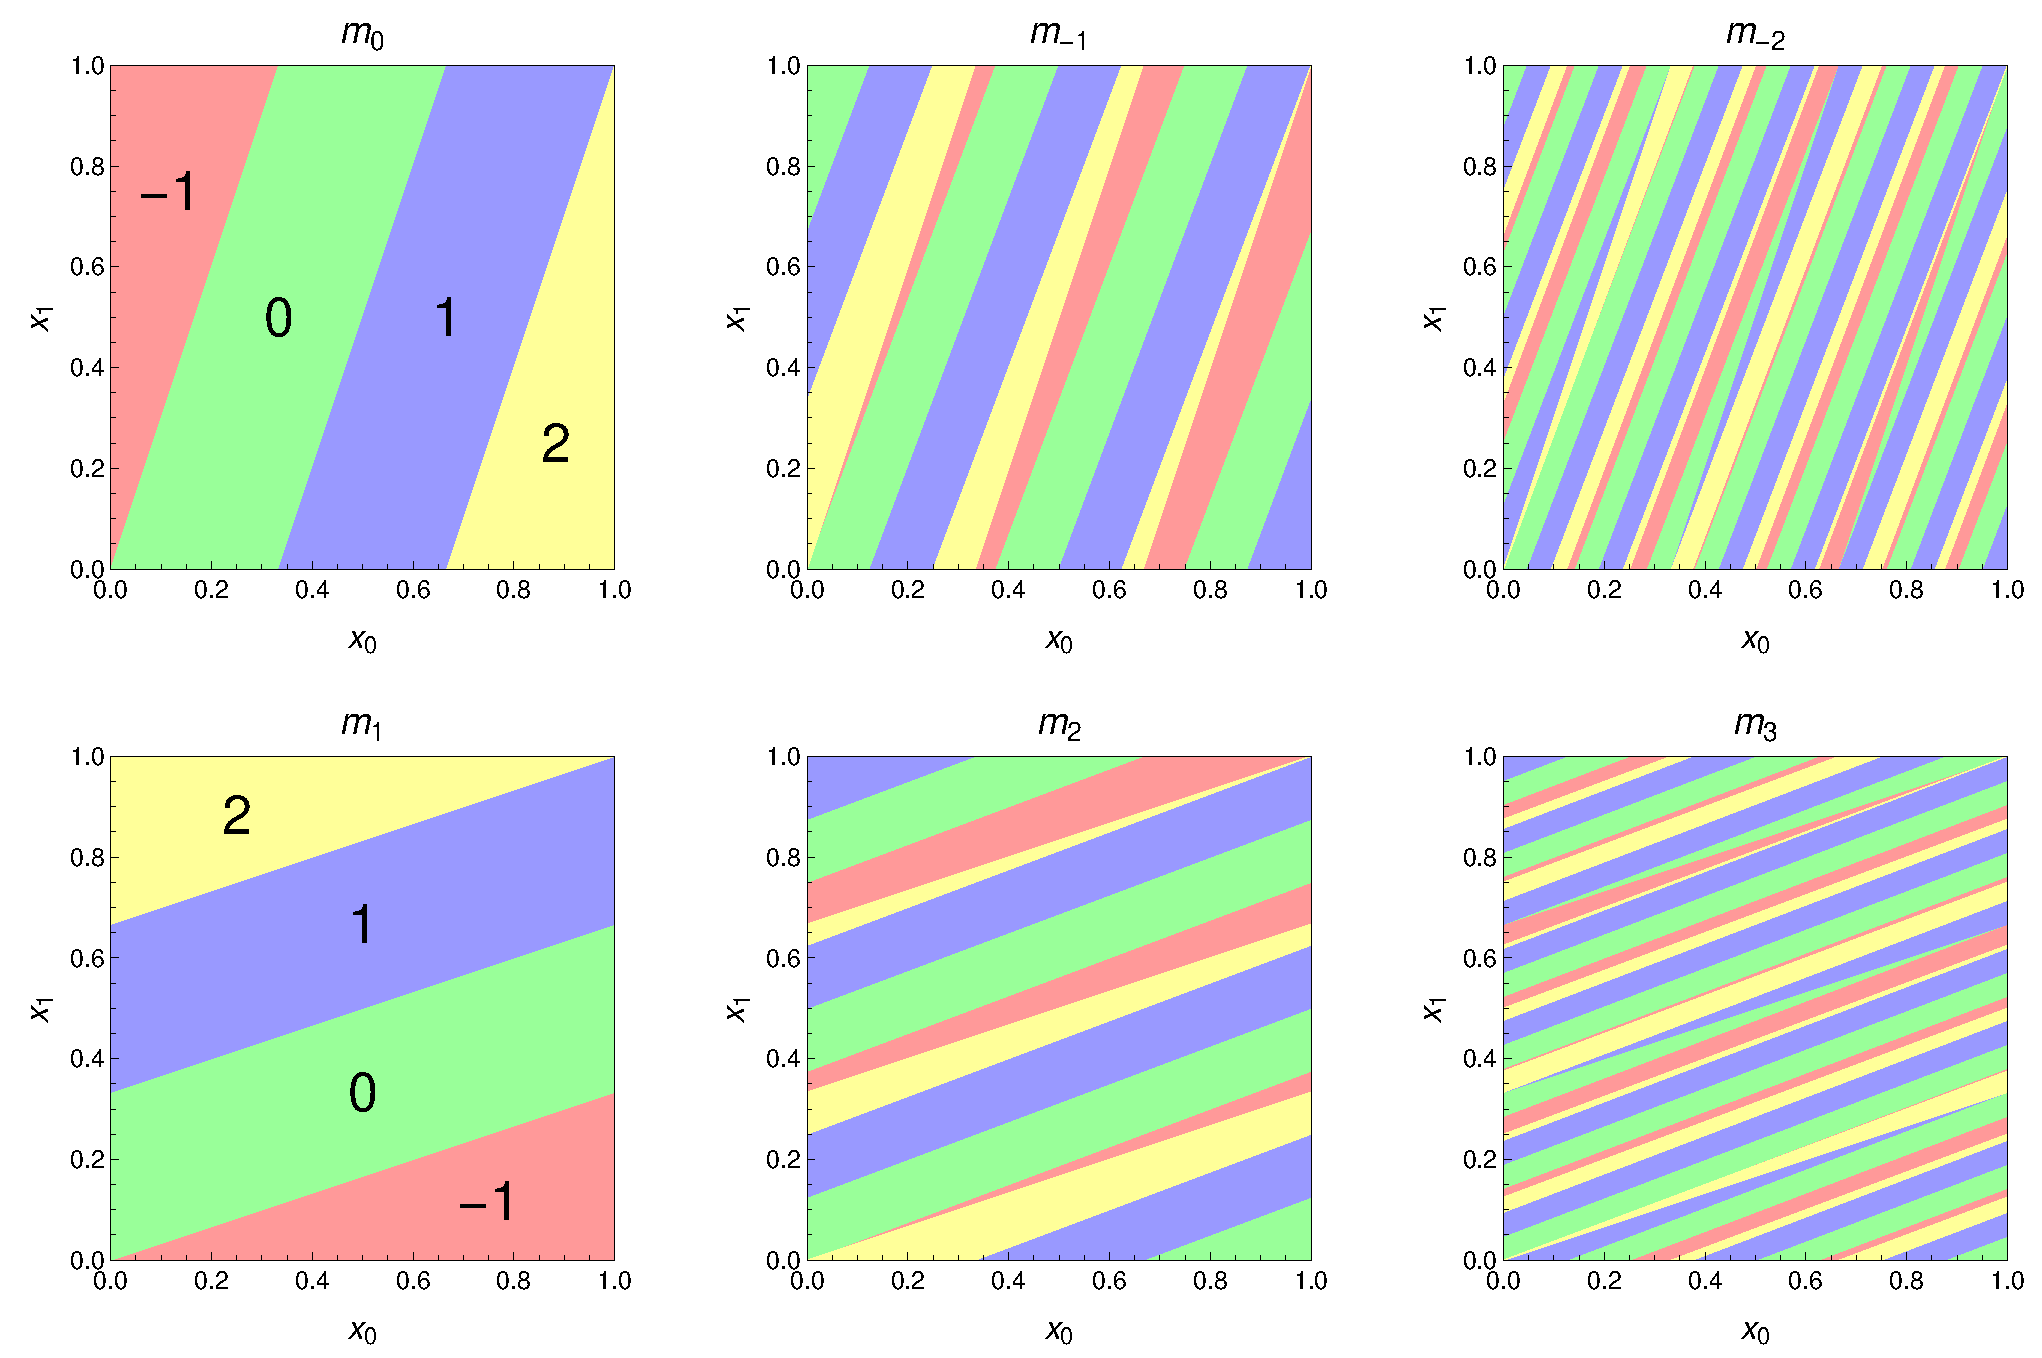
\includegraphics[width=0.95\textwidth]{SingleCat1Symbol}
	\caption{\label{fig:SingleCat1Symbol}
(Color online) $\ell = 1$ {\statesp s} on $(\ssp_{0},\ssp_{1})$  \statesp\ with respect
to symbols $\Ssym{t}$, $t = 0, -1, -2, 1, 2, 3$ for $s=3$. In each {\brick} values
of $\Ssym{t} = -1, 0, 1, 2$ are shaded with light red, green, blue, and yellow,
respectively, and each color has the same total area ($1/6$ for $\Ssym{t} = -1,
2$, $1/3$ for $\Ssym{t} = 0, 1$) in all {\brick s}. All boundary lines are straight
lines with rational slopes, while the slopes tend to irrational values set by
stable/unstable directions of the cat map exponentially fast in the limit $t
\rightarrow \pm\infty$.
	}
\end{figure}
%%%%%%%%%%%%%%%%%%%%%%%%%%%%%%%%%%%%%%%%%%%%%%%%%%%%%%%%%%%%%%%%%%

%%%%%%%%%%%%%%%%%%%%%%%%%%%%%%%%%%%%%%%%%%%%%%%%%%%%%%%%%%%%%%%%%%
\begin{figure}
	\centering
[the same plot as \reffig{fig:SingleCatPartit}]
	%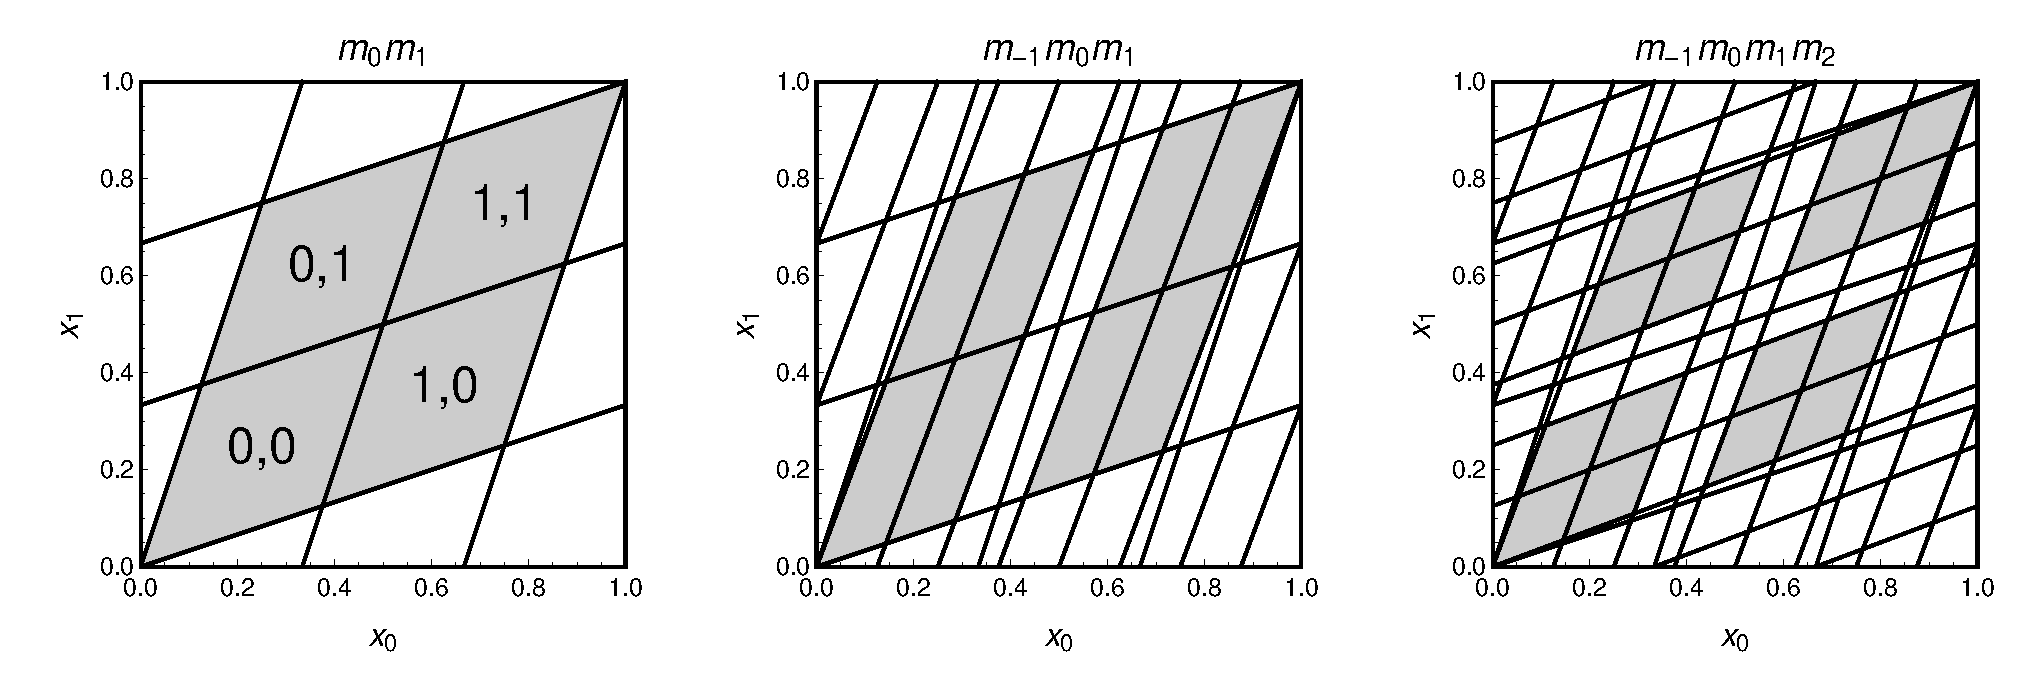
\includegraphics[width=0.95\textwidth]{SingleCatMultiSymbol}
	\caption{\label{fig:SingleCatMultiSymbol}
$\ell = 2, 3, 4$ {\statesp s} on $(\ssp_{0},\ssp_{1})$  \statesp\ for $s=3$, using {\brick s}
$\Ssym{0} \Ssym{1}$, $\Ssym{-1} \Ssym{0} \Ssym{1}$, and $\Ssym{-1} \Ssym{0} \Ssym{1} \Ssym{2}$ from the $\ell = 1$
diagrams. Shaded diamonds or rectangles correspond to sequences of all
interior symbols $(0, 1)^{\otimes \ell}$, having a total area of $4 \times
1/8$, $8 \times 1/21$, $16 \times 1/55$ respectively from left to right.
	}
\end{figure}
%%%%%%%%%%%%%%%%%%%%%%%%%%%%%%%%%%%%%%%%%%%%%%%%%%%%%%%%%%%%%%%%%%

Li Han text: ``
To generate such {\statesp} partitions, we start with length $\ell=1$. Consider
first the symbol $\Ssym{0} = s \ssp_0 - (\ssp_1 + \ssp_{-1}) =
\left\lfloor s \ssp_0 - \ssp_1 \right\rfloor$, where $\left\lfloor \cdots
\right\rfloor$ is the floor function. $\Ssym{0}$ has symbol boundaries
which are equally spaced parallel lines of slope $s$ and passing through
$(\ssp_0, \ssp_1) = (0, 0), (1, 1)$. We then look at the time-evolved
images of these symbol regions under forward map \refeq{eq:StateSpCatMap}.
The transformed region therefore means that at coordinate $(\ssp_{t+1},F
\ssp_{t+2})$ the point has symbol $\Ssym{t}$, which in turn implies that
when interpreted back to $(\ssp_{0},\ssp_{1})$  \statesp, a point is
associated with symbol $\Ssym{-1}$. As a result, we can generate all
length-1 {\statesp s} corresponding to symbols $\Ssym{t}$, $t = 0, \pm1,
\pm2, \cdots$ on the $(\ssp_{0},\ssp_{1})$  \statesp\ simply by applying
the forward map \refeq{eq:StateSpCatMap} or its inverse. We plot such
length-1 diagrams in \reffig{fig:SingleCatPartit} for symbols $\Ssym{0},
\Ssym{-1}, \Ssym{-2}$ (top), and $\Ssym{1}, \Ssym{2}, \Ssym{3}$ (bottom),
and call them different {\brick s}. Note that any of the {\brick s} can be used
to recover the 1-symbol measure $f_1(m)$ by calculating the total of
respective region areas, while with {\brick s} $\Ssym{0} = \left\lfloor s
\ssp_0 - \ssp_1 \right\rfloor$ and $\Ssym{1} = \left\lfloor s \ssp_1 -
\ssp_0 \right\rfloor$ the computations are the easiest, which have symbol
boundaries of slopes $s$ and $1/s$ respectively.

The fact that $\Msr(m
\in \Ai)$ are all equal and twice of $\Msr(m \in \Ae)$ is also obvious
from the $\Ssym{0}, \Ssym{1}$ {\brick s} of length-1 {\statesp s}.

A length-$\ell$ {\statesp} is then the superposition of any $\ell$
consecutive {\brick s} of length-1 diagrams, while a choice that is
symmetric about {\brick} $\Ssym{0}$ or $\Ssym{0}$ and $\Ssym{1}$ will
make the amount of calculations minimal. We have evaluated $\Msr(\m)$ up
to $\ell = 12$ from both \refeq{FreqDecomp} and symbolic diagrams for
$s=3$, $4$, $5$, and they are consistent. In \reffig{fig:SingleCatPartit}
we plot the symbolic diagrams for 2, 3, and 4 consecutive symbols using
{\brick s} $\Ssym{0,1}$, $\Ssym{-1,0,1}$, and $\Ssym{-1,0,1,2}$ of
\reffig{fig:SingleCatPartit}. Sequences of all interior symbols
correspond to congruent parallelogram regions whose opposite sides are
exactly parallel, and for even $\ell$ the regions are diamonds whose
sides are of equal length. Sequences of symbols from both \Ai\ and \Ae\
are not all admissible, which is the topic of next section. Here we note
that the corresponding regions of such sequences have general polygon
shapes and are not parallelograms, no matter which consecutive set of
{\brick s} we use.

%%%%%%%%%%%%%%%%%%%%%%%%%%%%%%%%%%%%%%%%%%%%%%%%%%%%%%%%%%%%%%%%%%%%%%%%
%    \PC{2016-12-27} {reuse this text from \reffig{fig:SingleCatPartit}? ``
All boundary lines are straight
lines with rational slopes, while the slopes tend to irrational values set by
stable/unstable directions of the cat map exponentially fast in the limit $t
\rightarrow \pm\infty$.
%    }
%%%%%%%%%%%%%%%%%%%%%%%%%%%%%%%%%%%%%%%%%%%%%%%%%%%%%%%%%%%%%%%%%%%%%%%%

From \refeq{FreqDecomp} the measure $\Msr(b)$ for a {\brick} $b =
\Ssym{1} \Ssym{2} \cdots \Ssym{\ell}$ is proportional to the area
of the polygon defined by inequalities (\ref{SquareCut1}).

The full list of measures $\Msr(\Ssym{1} \Ssym{2} \cdots \Ssym{\ell})$
has a tensor structure of tensor rank $\ell$ with each index running over
$\A$ and can be interpreted as a joint probability function.
''

Boris results.tex text: ``
whose lower left corner is the $(n,t)$ lattice site
\[
 \R_{nt} =\{(n+i, t+j) | i= 0, \dots, \ell_1-1, j= 0,\dots, \ell_2-2 \}
\,,
\]

It is straightforward to see that when \Mm\ is such that all symbols $\Ssym{z}$
belong to $\Ai=\{0,\dots,s-4\}$ then    \Mm\ is always admissible. By
positivity of  Green's function (see \refappe{sect:Green}) it follows
immediately that  $0 <\ssp_{z}$  while the condition
$\sum_{z'\in\integers}\gd_{zz'}=s-2$ implies that $\ssp_z\leq 1$.

''

Predrag text, recycle: ``
Here the piecewise linearity of the {\catlatt} enables us to go far analytically.
Essentially, as the cat map stretching is uniform, distinct admissible symbol
\brick s count all \brick s of a given shape (they all have the same
stability, and thus the same dynamical weight), and that can be accomplished
by linear, Green's function methods.
''

Predrag removed Boris poetry:
``
The  alphabet  separation into interior and external parts  nicely
illustrates  the  transition of the model from the correlated regime   to the
uncorrelated  Bernoulli process as parameter  $s$ in \refeq{LinearConn} tends
to $\infty$. Indeed, the number of external symbols in \Ae\ is fixed within a
given differential operator $\Box$  structure, while  the number of interior
symbols in \Ai\  grows linearly with the parameter $s$ controlling the
strength of chaos in a single map.   For {cat map} this transition can
be achieved by merely increasing the time step of time evolution. Increasing
the time step from $1$ to $2$ leaves the form of equation \refeq{OneCat}
intact, but renormalizes the  constant  $s\to s^2-1$.  This reflects the fact
that $\phi^2$  is more ``chaotic'' than  $\phi$. With an increase of  $k$
the map $\phi^k$ resembles more and more uncorrelated   Bernoulli process.
Similar transition can be observed  in the coupled  $\integers$ map lattices,
with a caveat that switch   from $\Phi$ to  $\Phi^k$ renormalizes  not only
the constant $s$, but   $\Box$  itself. The resulting equation of motion will
contain an  elliptic operator $\Box^{(k)}$ of higher order. Still,  it is
straightforward  to see that   the number of external symbols  is controlled
by  the order of the  operator $\Box^{(k)}$ which  grows linearly with $k$.
On the other hand, the number of interior symbols grows in the same way as
the constant  $s$ \ie, exponentially.
''

%%%%%%%%%%%%%%%%%%%%%%%%%%%%%%%%%%%%%%%%%%%%%%%%%%%%%%%%%%%%%%%%%%%%%%%%
%   \PC{2017-02-16} {
Replaced $N$ (for $N$ ``particles'') by $L$ (for spatial
extent) throughout
%    }
%%%%%%%%%%%%%%%%%%%%%%%%%%%%%%%%%%%%%%%%%%%%%%%%%%%%%%%%%%%%%%%%%%%%%%%%

\BGpost{2019-09-10}{
Old version, now replaced in results.tex by a more compact paragraph:

\medskip

To be specific, let \R\  be a   rectangular $[\ell_1\!\times\!\ell_2]$ region,
and let
\(
\Mm_{\R} % =\{\Ssym{z}\in \Mm | z\in \R \}
\)
be the  $[\ell_1\!\times\!\ell_2]$
\brick\ of \Mm\ symbols from
the alphabet $\A$.
Let
\(
\mathcal{N}(\Mm_{\R}|\Mm_{[L\!\times\!T]})
\)
be the number of times a given symbol {\brick} $\Mm_{\R}$ appears anywhere within
a much larger admissible symbol {\brick} $\Mm_{[L\!\times\!T]}$
cut out from a {\spt}ly infinite generic solution \Mm\ of the
\catlatt\ \refeq{LinearConn}.
The $d=1$ cat map is known to be fully hyperbolic and ergodic for $s>2$, with a
unique invariant natural measure $\Msr$  in the \statesp\
\refeq{eq:CatMapIntr} of the system.
The $d=2$  \catlatt\  is fully hyperbolic and ergodic for
$s>4$, see \refeq{qudreq}. In the language of spatially extended systems, we
assume that a steady state {\spt}ly chaotic solution is on average
{\spt}ly invariant, so the number of times a \emph{given} admissible
\brick\ $\Mm_{\R}$ shows up over a region $[L\!\times\!T]$ is expected to grow
linearly with the area $LT$. Hence a \emph{relative} frequency of the
occurrence of  the {\brick} $\Mm_{\R}$ can be defined as
\beq
f(\Mm_{\R}|\Mm_{[L\!\times\!T]})
    =
\frac{1}{LT}
\mathcal{N}(\Mm_{\R}|\Mm_{[L\!\times\!T]})
\,.
\ee{relFreqR}
With $L$ and $T$ increasing at comparable rates (for example,
take a square $[L\!\times\!T]$, with $L=T$), the ergodic measure of finding the
{\brick} $\Mm_{\R}$ across the infinite {\spt} domain is given by
\beq
\Msr(\Mm_{\R}) =
\lim_{L,T \to\infty}
f(\Mm_{\R}|\Mm_{[L\!\times\!T]})
\,,\qquad
\sum_{{\Mm_{\R}}} \Msr({\Mm_{\R}}) =1
\,.
\ee{relFreq}

\bigskip

For an ergodic system with a  unique invariant natural measure $\Msr$, the
limiting frequencies  $f(\Mm_{\R})$ are equal to the measures $\Msr( \pS_{\R})$
of the cylinder sets $ \pS_{\R}$, defined as sets of \statesp\ points $\Xx_{\R}$
having $\Mm_{\R}$ symbolic representation over the region \R. For this reason, we
sometimes refer, with a slight abuse of notation, to the frequencies
$f(\Mm_{\R})$ defined by \refeq{relFreqR} as measures of $\Mm_{\R}$ in the limit
$L,T \to\infty$, and denote them by $\Msr(\Mm_{\R})$ in what follows.
    }

\item[2016-11-20 Boris]
The {\spt} symbols follow from the Newtonian equations
in $d$ {\spt} dimensions
\bea
\Ssym{n,j} &=& (q_{n,j+1} -2 q_{n,j} + q_{n,j-1})
         + (q_{n+1,j}  -2 q_{n,j} + q_{n-1, j}) -  (s-4) q_{n,j}
        \continue
{\m} &=& [\Box + 2d\mathsf{1} -s\mathsf{1}]\, {\q}
\,.
\label{PC}
\eea

%As our ultimate goal is semiclassical quantization of a quantum many-particle
%system (or a quantum field theory),

%\PCpost{2017-01-03} {
%I changed the sign of $\Ssym{nt}$ in \refeq{CoupledCats},
%as in \refeq{LinearConn}, do all cats approve?
%    }
%\BGpost{2017-07-31}
%{Changed it back. Our present convention is the opposite one!}

    \PCpost{2017-02-16} {
To me, the Green's functions look strictly positive. Must harmonize
definitions \refeq{GreenFun0}, \refeq{GreenFun00}, \refeq{GreenFun000},
\refeq{LinearConn} and
\refeq{OneCat}, originating in Boris' flip-flop $\Ssym{t}\to-\Ssym{t}$

Is there a reference to Green's functions in terms of Chebyshevs?
    }
\BGpost{2017-08-02} {Yes,  and  it is OK with our present convention  -
Green's functions must be positive.}
    \BGpost{2017-08-02}{
%    I have checked the consistency of the symbol definitions ($m\to -m$
%    issue). Double check  might be needed in captions, but otherwise OK.
    Rule-of-thumb - internal symbols are non-negative, Green's functions
    are positive.}

\BGpost{2017-07-31}{
``As every Anosov automorphism is topologically conjugate to a linear cat
map ...'' Is it really true ?
}

    \PCpost{2017-08-11} {
That's what I read in some of the articles cited. But no need to say it
here, so now this is removed from our article.
    }

    \PCpost{2016-11-13}{ to all cats -
where we write \refeq{OneCat},
Percival and Vivaldi\rf{PerViv} write their Eq.~(3.6)
\(
(\Box +2 - s) \ssp_{t} = -b_t
\) %ee{PerViv3.6Bl}
so their ``stabilising impulses'' $b_t$  have the opposite sign to our
``winding numbers'' $\Ssym{t}$ (defined on $\ssp\in[0,1)$).\\
To all cats: keep checking that  after your flip of signs of $\Ssym{t}$'s
Eqs.~\refeq{LinearConn}, \refeq{OneCat}, \refeq{Coord} and \refeq{PC} are
consistent.
    }
\BGpost{2017-07-31}
{ Changed time ago. They should have the same sign as Percival and
Vivaldi i.e., our  $m$ are positive!}

%    \PCpost{2017-08-05}{dropped this: ``
%We illustrate this by first reviewing the $d=1$ case
%(introduced in \refref{PerViv}), but the focus of the paper is the $d=2$
%case (introduced in \refref{GutOsi15}).
%    ''}

%%%%%%%%%%%%%%%%%%%%%%%%%%%%%%%%%%%%%%%%%%%%%%%%%%%%%%%%%%%%%%%%%%%%%%%%%
%    \PCpost{2016-12-15} {
%%Definition \refeq{relFreq} is not normalized correctly.
%I worry a
%bit as whether it makes sense. It works for a single letter, $\R =
%[1\times 1]$. Have to argue that for larger \brick s
%\(
%   \mathcal{N}(\Mm_{\R}|\Mm_{[L\!\times\!T]})
%\)
%does not grow exponentially or
%as a power of $LT$? Perhaps obvious...
%    }
%    \BGpost{2017-07-29}{
%Looks like a misunderstanding here. I have tried to make the text more
%clear. We should distinguish between  frequencies in \refeq{LinearConn}
%and measures $\Msr(\Mm_{\R})$, at least on the level of definitions. They
%coincide for systems with unique ergodic measure.
%%and it is our assumption through the whole paper that this is the
%%case.(But we lack a mathematical prove of this. )
%For me  the normalization looks
%correct. Note that  $LT$ is  just the  total number of patterns within
%$\Mm_{[L\!\times\!T]}$ (minus boundary ``effects``).
%    }
%%%%%%%%%%%%%%%%%%%%%%%%%%%%%%%%%%%%%%%%%%%%%%%%%%%%%%%%%%%%%%%%%%%%%%%
   \PCpost{2017-08-11} {
I now get it. $LT$ is the area of \R. The  total number of \brick s
grows exponentially with the size of $\R$ and
is bounded from above by $(LT)^{|\A|}$.
You are saying that the number of
times a \emph{single} admissible \brick\ $\Mm_{\R}$ shows up over a region
$[L\!\times\!T]$ grows linearly with the area $LT$, and so does the
sum over frequencies of all distinct admissible \brick s ${\Mm_{\R}^{'}}$?
These ``frequencies'' are \emph{relative}, in the sense that correct
normalization is not \refeq{relFreq}, but
\beq
\Msr(\Mm_{\R}) = \frac{f(\Mm_{\R})}{
\sum_{{\Mm_{\R}^{'}}} f(\Mm_{\R}^{'})
            }
\,.
\ee{freqNormalized1}
    }
%%%%%%%%%%%%%%%%%%%%%%%%%%%%%%%%%%%%%%%%%%%%%%%%%%%%%%%%%%%%%%%%%%%%%%


    \PCpost{2017-08-05 }
    {Cylinder sets are subtle: if we were counting only {\em admissible}
$\Xx$, the cylinder set would be much smaller. But we almost never know
all inadmissible states.
\index{block!finite sequence}
\index{cylinder!set}
    }

 \BGpost{2017-07-31}
 {Li subsection {\em {\Brick s} of length $\ell$,}
% \label{sect:catGenerL}
 was siminos/cats/catGenerL.tex 2017-02-17, mostly
 contained repetitions of the previous stuff. Did not think we needed it. Few
 usable things  could be brought to other places. Agree?}
 \PCpost{2017-08-23}{Done.}

 \PCpost{2017-08-26}{Removed: ``
                                                \toCB
The term $\Box + 2 d\,\mathsf{1}$ is the standard statistical mechanics
diffusive inverse propagator that counts paths on a $d$\dmn\
lattice\rf{CBook:appendSymm}, and $-s\mathsf{1}$ is the on-site cat map
dynamics
(for the Hamiltonian formulation, see \refappe{sect:HamiltonCatLatt}).
        }

\BGpost{2017-08-05} {
Something unclear here (at least for me). ``The iteration of a map
$g(\ssp_{t})$ generates a group of  \emph{time translations}''.  Why
translations?   $g$ is a (time) map  acting  on all sites of lattice
independently (no interaction). Note: I think the models in \rf{PesSin88} and
\rf{BunSin88} are of the  same type. Both  can be thought of as products of
two maps: `` Interactions'' $\cdot$ ``Single particle propagations'' (i.e.,
product of $g$'s)
\\
{\bf 2017-09-04 Predrag}: You are right, I have rewritten that text now.
  }

    \PCpost{2017-08-28} {
For the Dirichlet (as opposed to periodic) boundary condition, which breaks
the translational symmetry, we take the very unphysical b.c. $\ssp_z=0$ for
$z\in\R$. Finite windows into turbulence that we describe by our symbol
\brick s never have such edges. Methinks...
    }
%%%%%%%%%%%%%%%%%%%%%%%%%%%%%%%%%%%%%%%%%%%%%%%%%%%%%%%%%%%%%%%%%%%%%%%%

\BGpost{2017-09-12}{
This equation
\bea
\ssp_{n, t+1}&=&p_{nt}+(s-3)\ssp_{nt} - (\ssp_{n+1,t} - 2\ssp_{nt} + \ssp_{n-1,t}) - {m}^\ssp_{n,t+1}
\continue
p_{n,t+1}&=&p_{nt} + (s-4) \ssp_{nt} - (\ssp_{n+1,t} - 2\ssp_{nt} + \ssp_{n-1,t}) - {m}^p_{n,t+1}
\,.
\label{eqmotion0}
\eea
seems wrong. We use \refeq{eqmotion}.
    }

    \BGpost{2017-09-14} {
Recall that (the Dirichlet) $\gd_{zz''}$ is a function of both $z$ and $z''$
and not just of the  distance between them $|z-z''|$.
    }

    \PCpost{2017-09-04}{
``integer $s>4$'' is not the correct condition, for $d=2$ $s=4$ is presumably
already hyperbolic. To add to the confusion, in his report Adrien computes
for $s=3$, the case with no interior alphabet symbols. So $s>2$ is the
correct hyperbolicity condition for all $d$?
Give the correct condition on $s$, explain it.
    }

\BGpost{2017-09-12}{
Here are the  answers to  this and co. questions over the paper.
\begin{enumerate}
  \item
The system is uniformly (fully) hyperbolic for  $s>2d$. This means all
eigenvalues of linearized map  (see  \refeq{qudreq}  for $d=2$) are  either
$|\ExpaEig|<1$  (stable subspaces)  or $|\ExpaEig|>1$ (unstable subspaces).
  \item
For $s=2d$ the system is partially hyperbolic. This means everything as above
except two  Lyapunovs for  which   $\ExpaEig=1$ (neutral subspaces).
  \item
For $|s|<2d$  system is non-hyperbolic. Apparently for everything in this
paper 1 $\&$ 2 is OK. But
  \item
drastically changes everything (suspect  a phase transition in physics jargon
i.e., non-unique SRB measure). So whatever we consider  in the paper should
be for $s\geq 2d$.
\end{enumerate}
    }

 \BGpost{2017-09-14} {
A comment on $s=2d$ case (do not know how much of it we need for the paper).
Our results in this paper require in principle  $s>2d$ (all Lyapunovs are
positive). However certain things still work (by whatever reason)  for $s=2d$
as two figs in \refsect{sect:catLattEntropy} show. In this case the total
momentum $\sum_{n=1}^L p_{nt}$ is preserved. This can be seen from the
invariance of \refeq{LinearConn} under   translation  $x_{nt}\to
x_{nt}+\alpha$. So the system is not ergodic  and linear encoding is not one
to one (different trajectories might have the same symbolic representation).
However, it is (probably)  ergodic on the shell   $\sum_{n=1}^L p_{nt}=const.$
This is probably the reason why  our formulas for frequencies of  $\Mm_{\R}$
still work.
 }

\BGpost{2017-09-26}{Dropped this:
``
with the corresponding probability of occurrence of a fixed symbol
{\brick} $\Mm_{\R}$ given by
\[
\Msr(\Mm_{\R}|\Mm_{[L\!\times\!T]}) =
\frac{f(\Mm_{\R}|\Mm_{[L\!\times\!T]})}
     {
\sum_{{\Mm_{\R}^{'}}} f(\Mm_{\R}^{'}|\Mm_{[L\!\times\!T]})
     }
\,,\qquad
\sum_{{\Mm_{\R}}} \Msr({\Mm_{\R}}|\Mm_{[L\!\times\!T]}) =1
\,,
\]  %\ee{freq2measure}
where the sum goes over all distinct admissible {\brick s}
${\Mm_{\R}^{'}}$.''

The point is that
\[
\sum_{{\Mm_{\R}}}\mathcal{N}(\Mm_{\R}|\Mm_{[L\!\times\!T]})= LT - \mbox{
``Terms linear in L and T''}.
\]
So no need in an artificial normalization -
normalization in  \refeq{relFreq} would follow anyhow.
}

 \BGpost{2017-09-14} {Replaced this eq.
\beq
\Mm\cup\partial\R
    =
\left[\begin{array}{c}
\ssp_{12}   \\
\ssp_{01}~\Ssym{11}~\ssp_{21} \\
\ssp_{10}   \\
\end{array}\right]
    =
\left[\begin{array}{c}
\ssp_{2}   \\
\ssp_{1}~\Ssym{11}~\ssp_{3} \\
\ssp_{4}   \\
\end{array}\right]
\ee{block1x1border}
by the first plot in \reffig{fig:block2x2}.
 }

    \PCpost{2016-11-15, 2017-08-28} {
Note: When I look
at the intersection of the diagonal with the partition strips in by
inspecting \reffig{fig:SingleCatPartit}, I find that the Fibonacci
numbers 1,2,3,5, ... give the numbers of periodic points, in agreement with
the \AW\ Markov partition. So the linear
code is not a generating partition, but \po s do the right thing anyway.
    }

\PCpost{2018-04-05 to Adrien from}{
I think \reffig{fig:AKScloseActSp} is really hard to explain to a reader;
why these axes, how did all points get mapped into the same unit square,
why there are huge empty swaths - all stuff that distracts from the
main point which is that $x_z$'s within the center of the shared symbol \brick\
are exponentially close.
    }

\PCpost{2018-04-05}{
I think we can simplify this greatly, using the fact that the (damped)
{\sPe} \refeq{LinearCatLatt} is linear, so one can subtract
patterns in order to visualize their distance.

In order to have a 2\dmn\ visualization for each \brick,
color the symbol $\Mm_j$ $[\speriod{1}\!\times\!\speriod{2}]$ \brick\ with discrete
color alphabet \Ai, as in \reffig{fig:AKScloseActSymb},
and the corresponding state $\Xx_j$ $[\speriod{1}\!\times\!\speriod{2}]$ \brick\
with colors chosen from a continuum color strip.

As this is a linear problem, you can also represent closeness of two
$[\speriod{1}\!\times\!\speriod{2}]$ \brick s by using this coloring scheme for
$\Mm_2-\Mm_1$ and $\Xx_2-\Xx_1$.
%To find the closest ``distance'' between
%2-tori, you will have to go through all cyclic permutations of the second one
%to align it optimally
%(or, if you understand ChaosBook course, you'll have to `slice').

For pairs of distinct 2-tori which share the same region of $\Ssym{z}$'s, or a
single 2-torus in which the same region of $\Ssym{z}$'s appears twice, the
states $\ssp_z$ in the center of the region should be exponentially close,
in order to demonstrate that they shadow each other.

So, replace \reffig{fig:AKScloseActSp} by
(a) $\Mm_2-\Mm_1$ from \reffig{fig:AKScloseActSymb} (it will be all the same
    color in the shared region), and
(b) plot $\Xx_2-\Xx_1$. Mark the lattice point $z$ with the minimal value of
    $|x^{(2)}_z-x^{(1)}_z|$ on this graph, and in the text state the minimal value of
    $|x^{(2)}_z-x^{(1)}_z|$.
    You can also state the mean Euclidean (or L2) distance between the
    two \twots:
\beq
d_{\Xx_2-\Xx_1} =
         \left(\frac{1}{LT} \sum_z (x^{(2)}_z-x^{(1)}_z)^2\right)^{1/2}
\,,
\ee{twotsDist}
or distance averaged over the lattice points restricted a region \R.
\\ \textcolor{blue}{(taken care of by AKS)}
    }

\AKSpost{2018-04-13}{
After reconstructing the orbits separately, I plotted the distance
between the positions in $(q,p)$ space for each lattice site $z$, see
the new \reffig{fig:AKSs7dist}, meant to replace the current
\reffig{fig:AKScloseActSp}.
\color{red}{Still have to use sensible color ranges,
and compute} \reffig{fig:AKSs7dist}\,(b).
%%%%%%%%%%%%%%%%%%%%%%%%%%%%%%%%%%%%%%%%%%%%%%%%%%%%%%%%%%%%%%%%%%%%%%%
\begin{figure}
\begin{center}
(a) 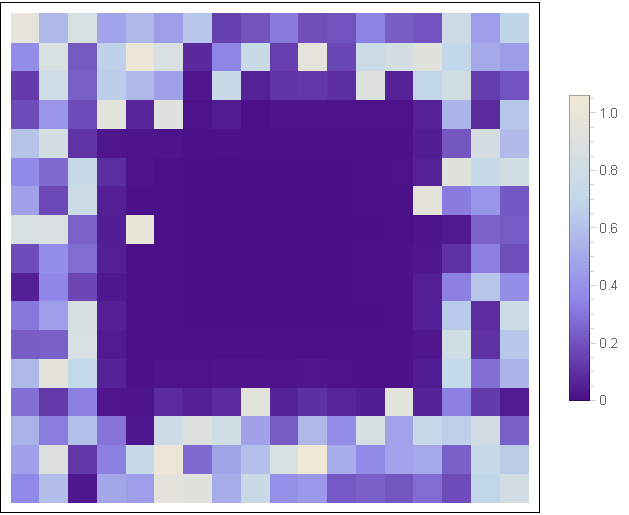
\includegraphics[width=0.45\textwidth]
{AKSs7distM1M2} %\hspace{0.7cm}
(b) 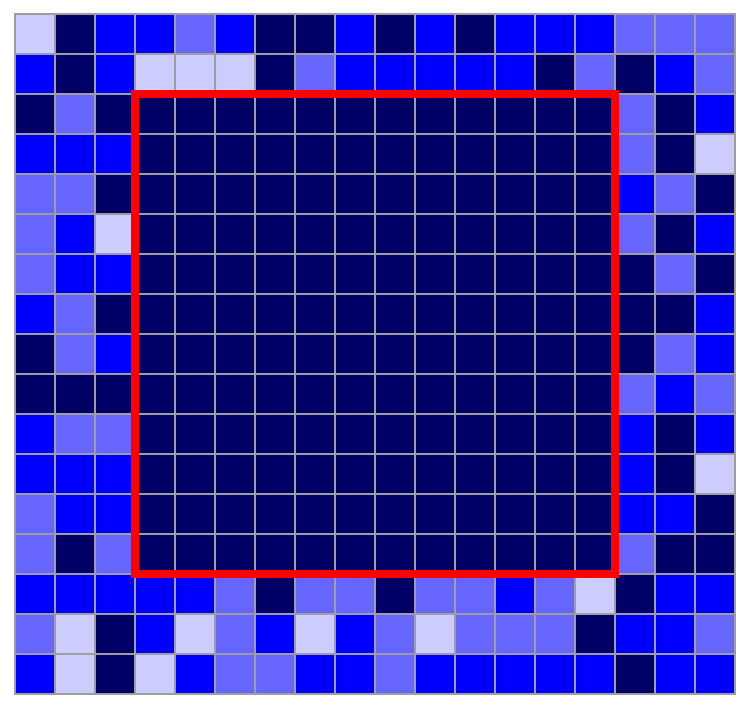
\includegraphics[width=0.37\textwidth]
{AKSs7distM1M2log}
\end{center}
\caption[]{
(Color online)
    (a)
\(\Xx_{2,z}-\Xx_{1,z}\,,\)
the site-wise distance between the \twots\ fields corresponding to the
two $[18 \times 18]$ \brick s
$\Mm_{1}$, $\Mm_{2}$ (colored tiles) of
\reffig{fig:AKScloseActSymb}\,(a,b).
    (b)
The plot of the site-wise symbol difference
\(
|\Mm_{2,z}-\Mm_{1,z}|
\)
 of  \reffig{fig:AKScloseActSymb}\,(b) and (b)
(for a better visualization, see \reffig{fig:AKSs7distupdated}).
}
\label{fig:AKSs7dist}
\end{figure}
%%%%%%%%%%%%%%%%%%%%%%%%%%%%%%%%%%%%%%%%%%%%%%%%%%%%%%%%%%%%%%%%%%%%%%%
\\ \textcolor{blue}{(taken care of by AKS)}
}

\PCpost{2018-04-13 to Adrien from}{
Also of interest might be the color-coded plot of value of $x_{q,p}$ for at
least one of them. Would be nice to check -at least once- whether there is
any relation to the corresponding  $m_{q,p}$ (probably there is no relation).

We'll have to rethink coloring (should be the same as  $m_{q,p}$, more or less).

As the distance decreases exponentially towards the center, you probably want
a color plot of
    $\ln |\ssp_{q,p}^{(2)} - \ssp_{q,p}^{(1)}|$
to resolve the small distances towards the center of the square.
\\ \textcolor{blue}{(taken care of by AKS)}
    }

%%%%%%%%%%%%%%%%%%%%%%%%%%%%%%%%%%%%%%%%%%%%%%%%%%%%%%%%%%%%%%%%%%%%%%%
\begin{figure}
\begin{center}
(a) 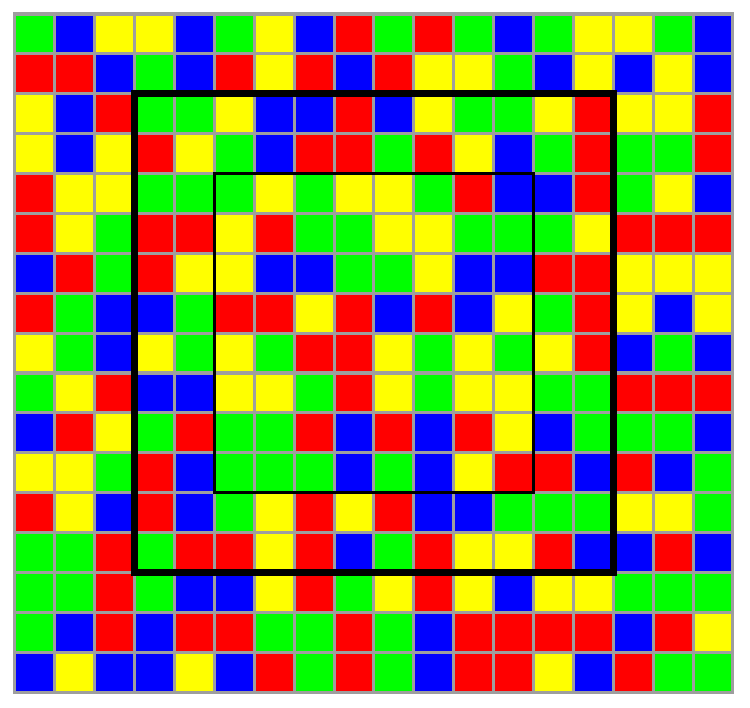
\includegraphics[width=0.45\textwidth]
{AKSs7colrBorderM1} %{AKSs7BlockBorderM1} %\hspace{0.7cm}
(b) 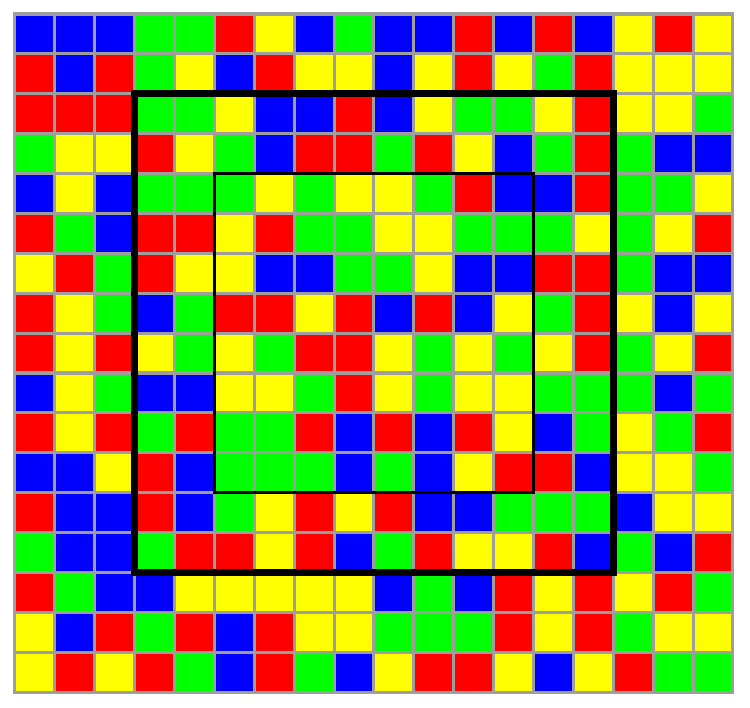
\includegraphics[width=0.45\textwidth]
{AKSs7colrBorderM2} %{AKSs7BlockBorderM2}
\end{center}
\caption[]{\label{fig:AKScloseActSymb}
\PCedit{Figure nixed by Boris 2019-08-21, replaced by digits
\reffig{fig:BGcloseActSymb}.}
%(Color online)
Symbolic representation (colored tiles) of two
$[L\!\times\!T] = [18 \times 18]$
{\twot} solutions of
\refeq{CoupledCats},
$s=7$,
that shadow each other within the shared
\brick\ $\Mm_{\R}=\Mm_{\R_{0}} \cup \Mm_{\R_{1}}$ (blue).
The symbols within \R, drawn randomly from the interior alphabet \Ai, are
the same for both solutions;
the symbols outside \R, also drawn randomly from \Ai, differ.
The shared \brick\ $\R=\R_{0} \cup \R_{1}$ is split into the interior region
$\R_{0}$ (bold blue) and the border strip $\R_{1}$ (blue).
%  AKS 2019-09-10
% (a) and(b) are in fact the color code \brick s a smaller size system than
% the one we use now in the main TEXT.
    }
\end{figure}
%%%%%%%%%%%%%%%%%%%%%%%%%%%%%%%%%%%%%%%%%%%%%%%%%%%%%%%%%%%%%%%%%%%%%%%

% \BGpost{2019-08-21} { % 2019-08-26 PC
%I prefer digits \reffig{fig:BGcloseActSymb}  rather than color
%\reffig{fig:AKScloseActSymb} for two reasons. Minor issue - colors are
%visible only online, slightly  more serious issue - colors will require a
%color map (to connect them with the code) = additional intermediate
%level. It also makes things more homogeneous = helps to understand
%\reffig{fig:AKSs13TwoBlock1} etc.
%\\ {\bf  implemented PC}
%\\ \textcolor{blue}{(taken care of by AKS)}
%    }

\BGpost{2017-08-02}
    {The representation \reffig{fig:BGcloseActSymb} has changed from
    digits to colors \reffig{fig:AKScloseActSymb}
    ({\bf PC} 2019-08-26 reverted this figure to digits).
    \\
    Was it try and see, or is it going to stay? In my
    opinion it is more colorful, but less informative. The reason is a)
    digits are directly $m_{nt}$ - no need to translate colors into
    numbers + make sense without  colors (on line). b) the encounters
    (regions with the same coding)   can be visualized   by coloring.}
    \PC{2017-08-11}
    {Well, that's a bit subjective - it is unintelligible to a human eye
    either way. I would keep this one figure as an illustration that
    color coding is an alternative to number coding.
    \\ \textcolor{blue}{(taken care of by AKS)}
}


 \BGpost{2019-08-21} { % 2019-08-26 PC
Now that we got rid of the color \reffig{fig:AKScloseActSp}, there's no
point in having two different colors in \reffig{fig:BGcloseActSymb} for
the overlapping regions of symbols, light blue for the outer region
called $\R_{1}$  in the paper, dark blue for the inner one called
$\R_{0}$.
\\ {\bf toDo}
\\ \textcolor{blue}{(taken care of by AKS)}
    }

 \BGpost{2019-08-21} {	
I like including the differences plot \reffig{fig:AKSs7dist}
or \reffig{fig:AKSLPS12}
(we have something similar in Our Paper\rf{GutOsi15} with Vladimir
Osipov)
{\bf (implemented PC 2019-08-27)}.\\
It should be included as addition to \reffig{fig:BGcloseActSymb}, and not
as substitution to it (it substitutes \reffig{fig:AKScloseActSp}, now
removed from the paper). Without \reffig{fig:BGcloseActSymb} it would be
difficult to digest and explain its content.}

\AKSpost{2019-10-30}{
I think by now we agreed we would keep the digits figure only. The
figures of symbolic difference (\reffig{fig:AKSs7dist}) and of symbolic
coloring (\reffig{fig:AKScloseActSymb}) are either outdated or ugly. We
can toss them out of the blog. \reffig{fig:AKSsymbol} and
\reffig{fig:AKScloseActSp} could be moved to another appendix. We could
also move \reffig{fig:AKSs7distupdated} to another appendix, as it is the
most recent ``difference of symbols" figure.\\
\textcolor{blue}{(taken care of by AKS)}
    }

 \PCpost{2019-08-27} {
If you mean ``metric distances'' of \GO\ figures A3 and C2, that is quite
different than our log(distance) plots. Problem is that \GO\ measure
Eucliden distance between symplectic phase-space points, not a meaningful
distance. Would have to subtract actions, but this is not a thing for
this paper...
    }

\AKSpost{2019-08-21} {
You mean \reffig{fig:AKSs7dist} here in \texttt{GHJSC16blog.tex}, \ie,
\reffig{fig:AKSLPS12}\,(a) which is the log of the norm of the
difference of the two trajectories in \statesp? I agree that if
anything, \reffig{fig:AKSLPS12}\,(a) should substitute
\reffig{fig:AKScloseActSp} and not \reffig{fig:BGcloseActSymb}.
What do you think on the updated color pattern,
\reffig{fig:AKSLPS12}\,(b)?
\\ \textcolor{blue}{(taken care of by AKS)}
    }

%\PCpost{2019-08-21} {
%Moved \reffig{fig:AKScloseActSp} from the  paper to here, replaced
%it by \reffig{fig:AKSLPS12}.
%                    }

 \BGpost{2019-08-26} {
Still not good enough. The coloring is too jumpy.   It should range from
white or light blue to dark blue. For a  more reasonable coloring  of
this type see figure~14 from Our Paper\rf{GutOsi15} \arXiv{1503.02676}.
Maybe also the periods of tori L, T  should be larger to make things
smoother.
%\\ {\bf toDo}
\\ \textcolor{blue}{(taken care of by AKS)}
        }

 \AKSpost{2019-08-21} {
 We still need the two symbolic representation figures in
\reffig{fig:BGcloseActSymb}.
In \reffig{fig:AKSsymbol} I have regenerated those symbolic
representation as numbers instead of colors, as an alternative to
\reffig{fig:BGcloseActSymb}. Which one do you prefer?
%\\ {\bf toDo}
\\ \textcolor{blue}{(taken care of by AKS)}
        }

 \BGpost{2019-08-21} {	
For \reffig{fig:RJsymbol} - a different coloring pattern is indeed needed
+ the size of the figures (a), (b) should be the same.
\\
{\bf AKS}
I agree. Except for the size, which should be the same as the current
\reffig{fig:BGcloseActSymb}\,(a).
\\ {\bf toDo}
\\ \textcolor{blue}{(taken care of by AKS)}
    }

%%%%%%%%%%%%%%%%%%%%%%%%%%%%%%%%%%%%%%%%%%%%%%%%%%%%%%%%%%%%%%%%%%%%%%%
\begin{figure}
\begin{center}
(a) 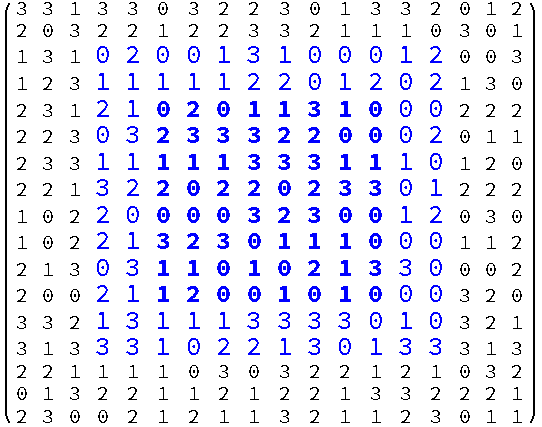
\includegraphics[width=0.45\textwidth]{AKSsymbol1}
%{AKSs7BlockBorderM1} %\hspace{0.7cm} %color: {AKSs7colrBorderM1}
(b) 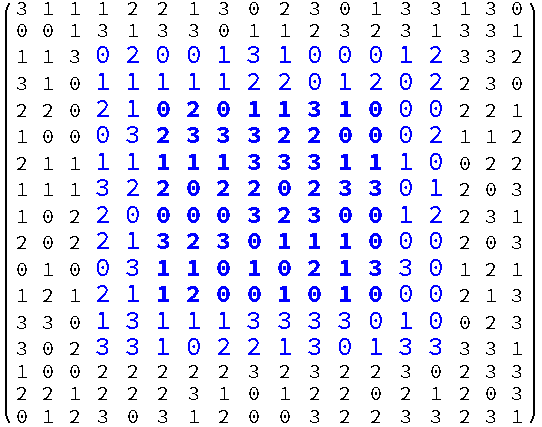
\includegraphics[width=0.45\textwidth]{AKSsymbol2}
%{AKSs7BlockBorderM2}                 %color: {AKSs7colrBorderM2}
\end{center}
\caption[]{
(Color online)
Symbolic representation (numbered tiles) of two
$[L\!\times\!T] = [18 \times 18]$
{\twot} solutions of
\refeq{CoupledCats},
$s=7$,
that shadow each other within the shared
\brick\ $\Mm_{\R}=\Mm_{\R_{0}} \cup \Mm_{\R_{1}}$ (blue).
The symbols within \R, drawn randomly from the interior alphabet \Ai, are
the same for both solutions;
the symbols outside \R, also drawn randomly from \Ai, differ.
The shared \brick\ $\R=\R_{0} \cup \R_{1}$ is split into the interior region
$\R_{0}$ (bold blue) and the border strip $\R_{1}$ (blue).
}
% in GHJSC16.tex: {fig:BGcloseActSymb}  %in blog, color: {fig:AKScloseActSymb}
\label{fig:AKSsymbol}  %in blog, color: {fig:AKScloseActSymb}
\end{figure}
%%%%%%%%%%%%%%%%%%%%%%%%%%%%%%%%%%%%%%%%%%%%%%%%%%%%%%%%%%%%%%%%%%%%%%%

%%%%%%%%%%%%%%%%%%%%%%%%%%%%%%%%%%%%%%%%%%%%%%%%%%%%%%%%%%%%%%%%%%%%%%%
\begin{figure} % PC 2019-08-27 replaced by \reffig{fig:AKSLPS12}
\begin{center}
(a) 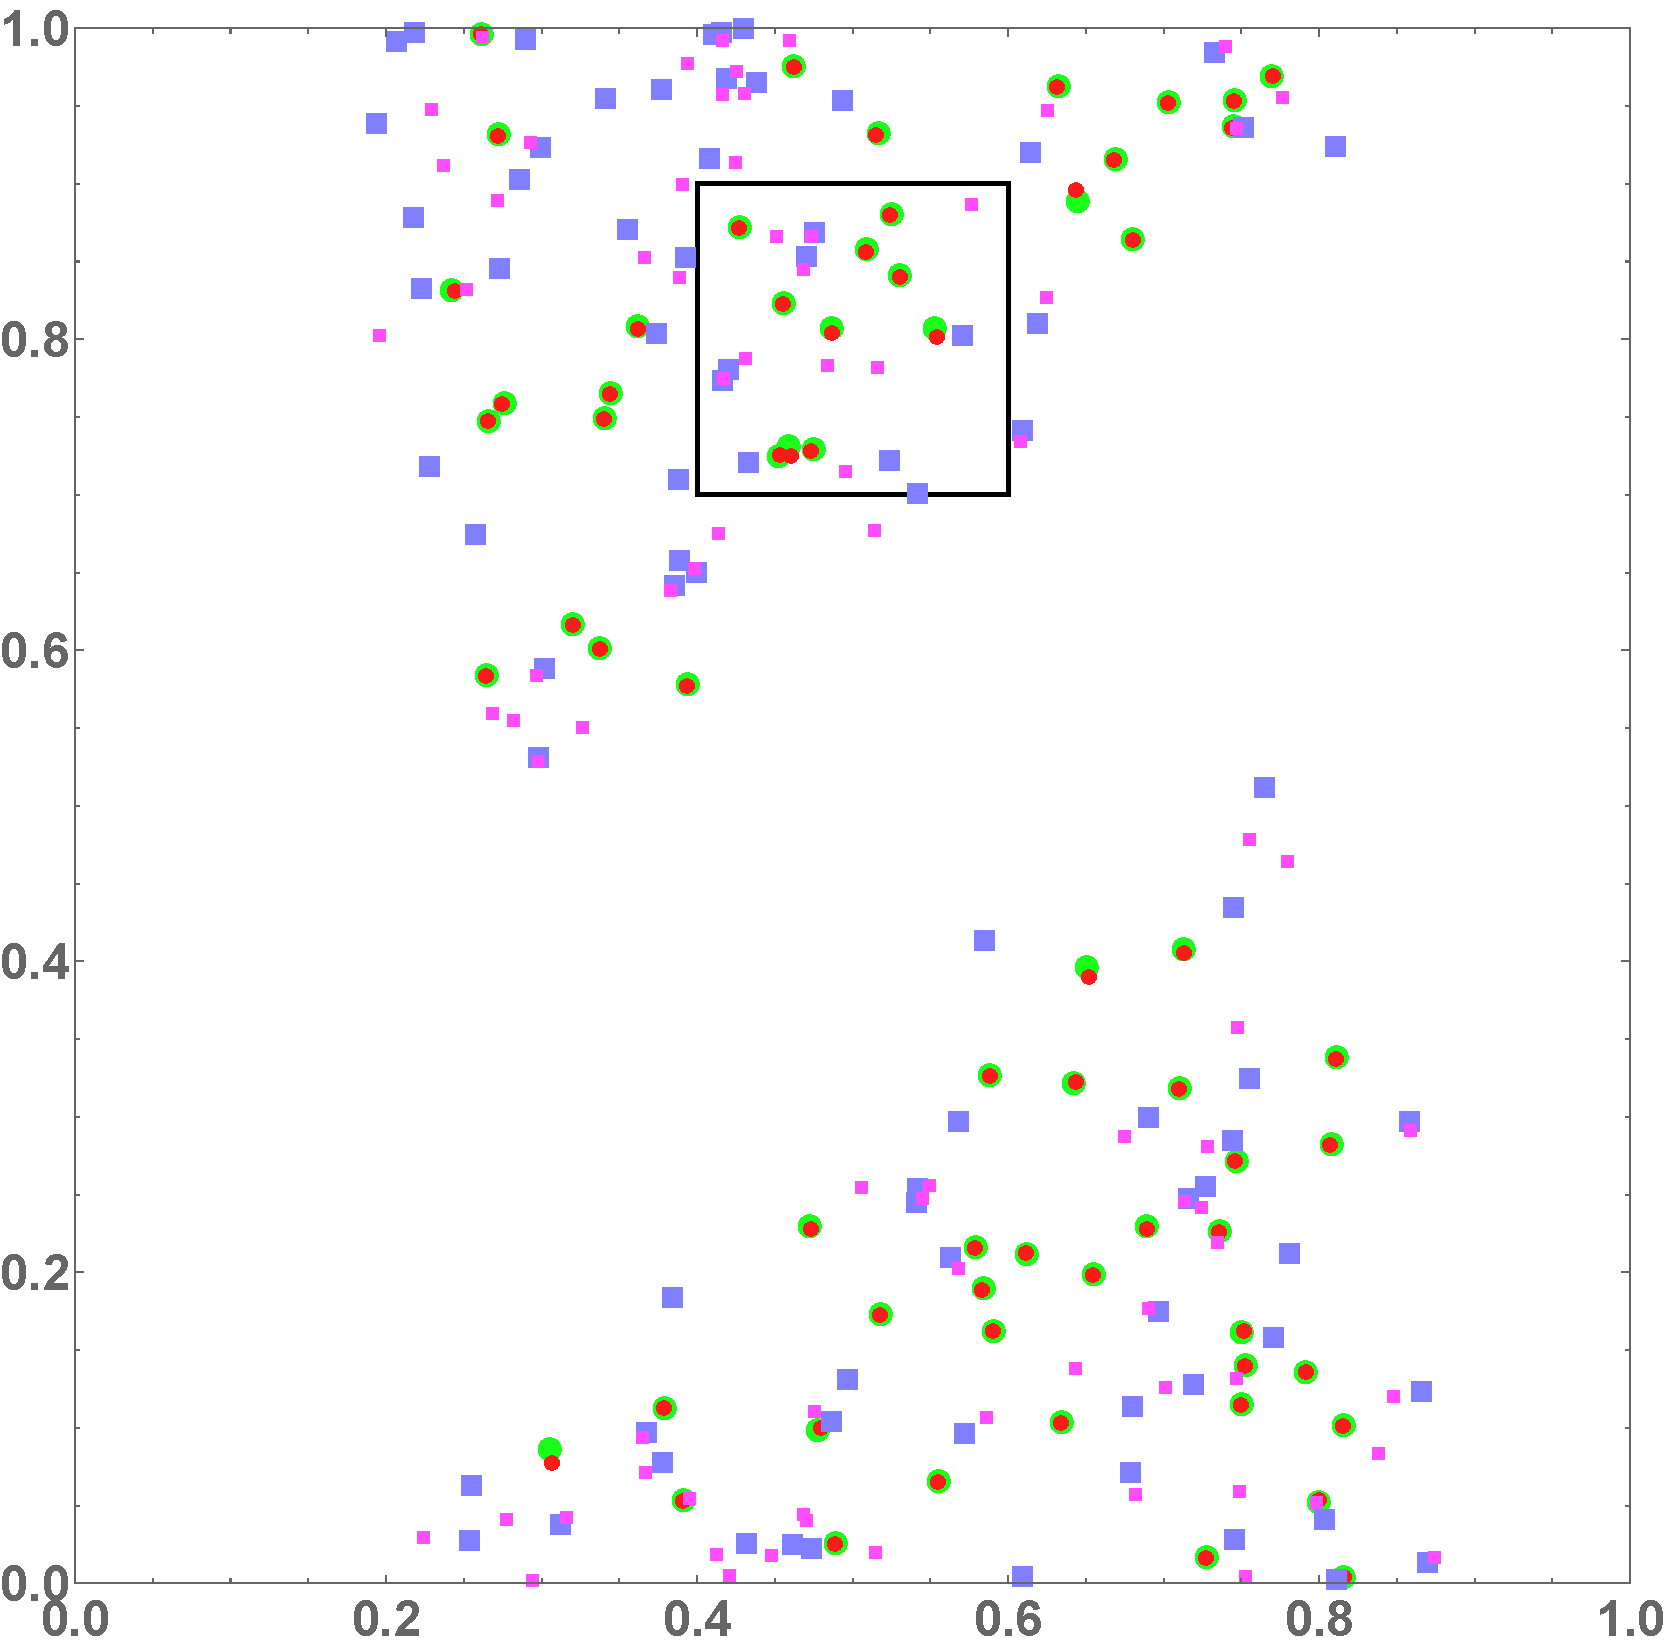
\includegraphics[width=0.42\textwidth]
{AKSs7BlockBorderG1}
\hspace{1ex}
(b) 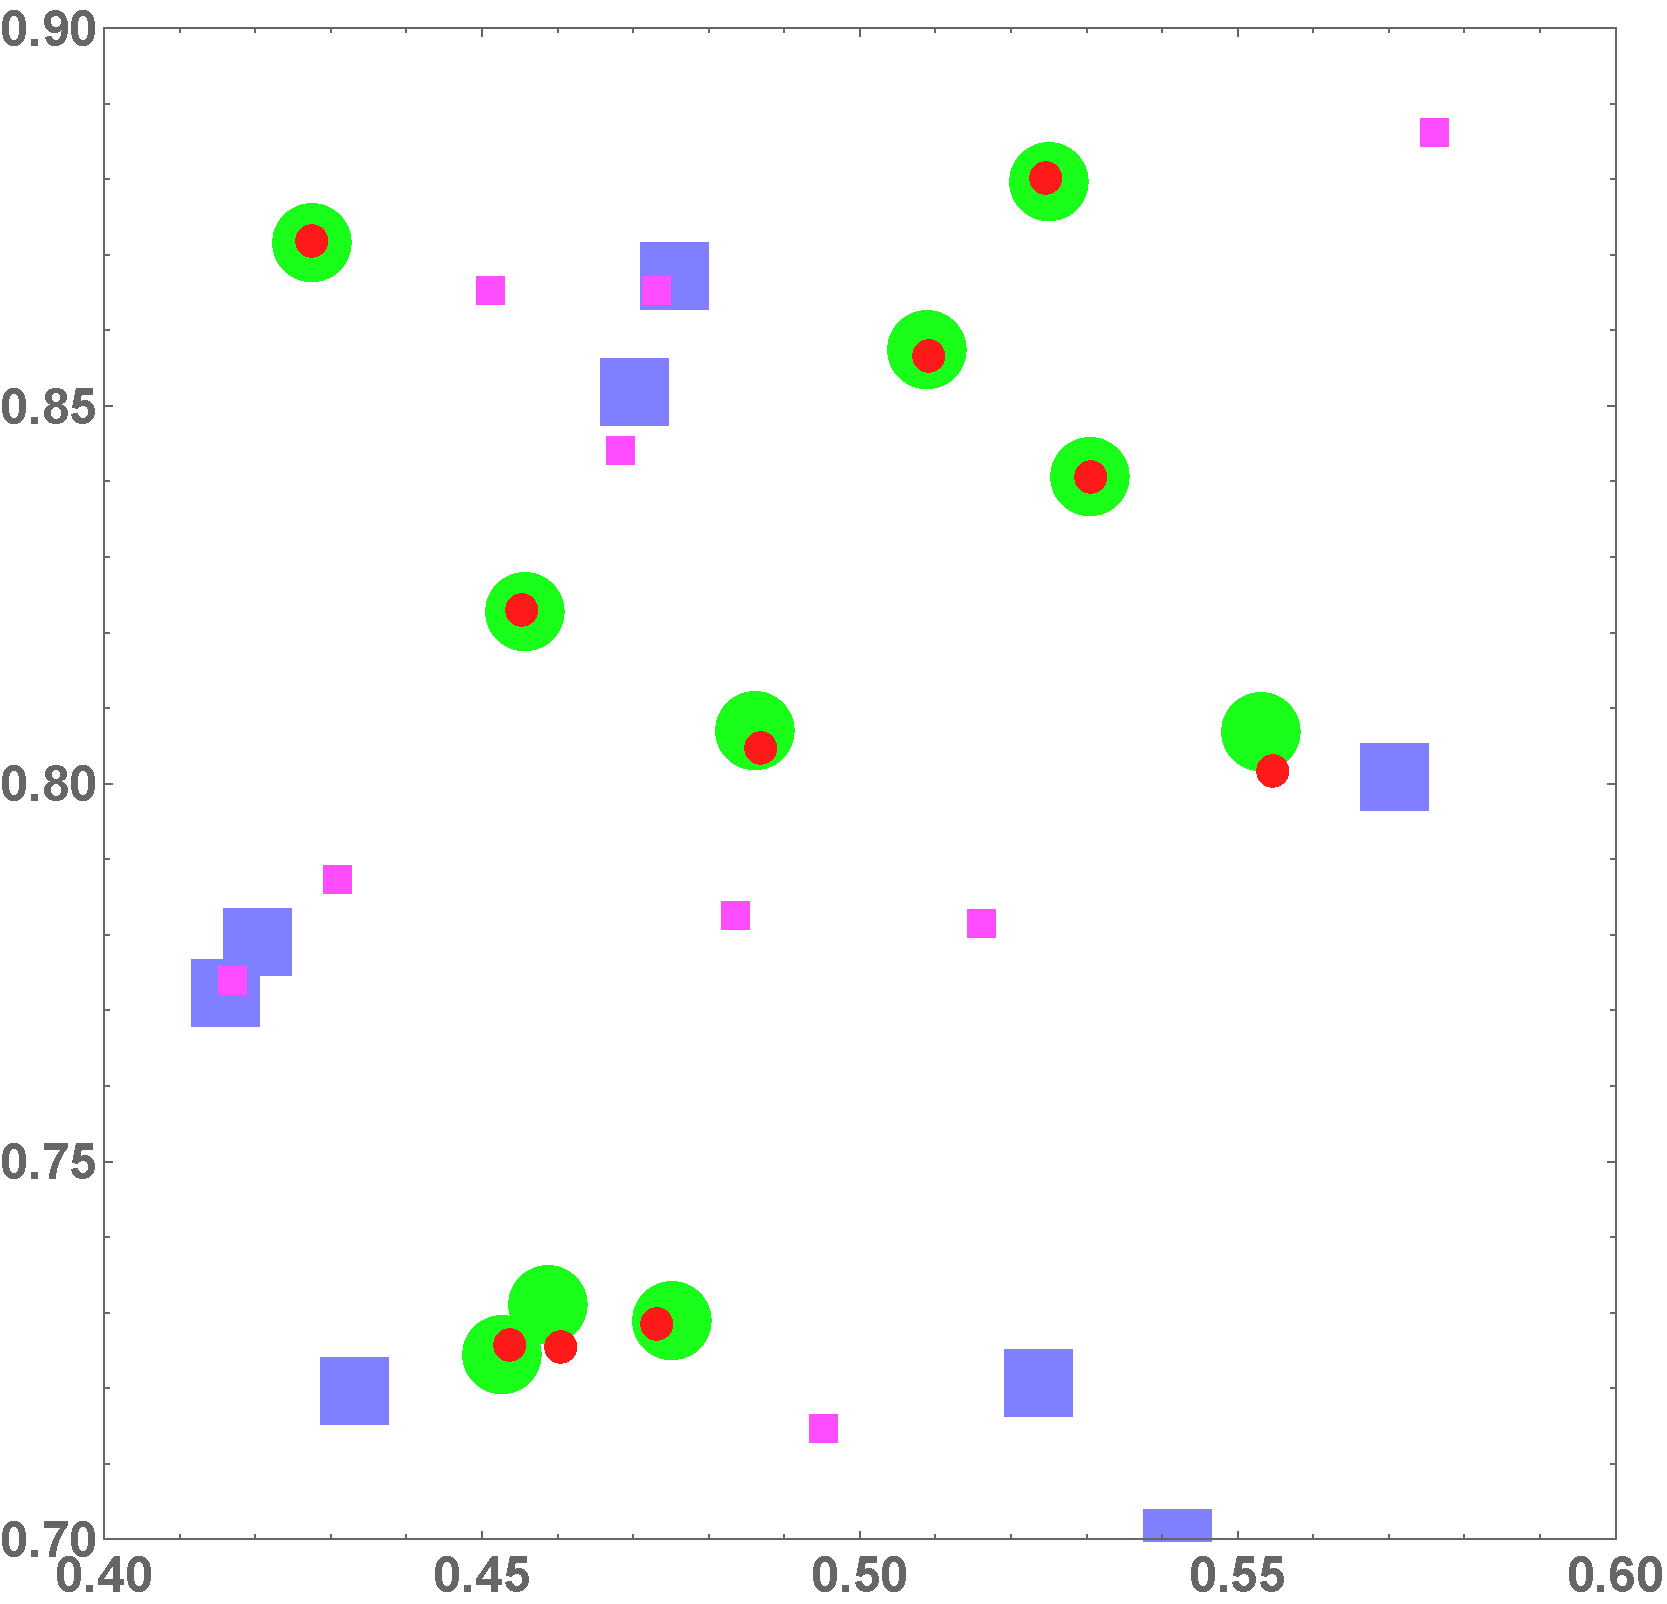
\includegraphics[width=0.43\textwidth]
{AKSs7BlockBorderG2}
\end{center}
\caption[]{
(Color online) (a) Phase space representation $(q^{(i)}_z,
p^{(i)}_z)$, where $i=1,2$  refers to the two \twots\ of
\reffig{fig:AKSsymbol}. (b) A zoom   into small rectangular area shown
on the left. The \statesp\ is covered only partially, as symbols in {\brick
s} $\Mm$ are restricted exclusively to the interior alphabet.
Only data for  $z=(n,t)\in \R$
are shown in the figure. The centers of red (small) circles  and green
(large) circles  are  the points $(q^{(i)}_z, p^{(i)}_z)$  of the first
($i=1$) and the  second ($i=2$) \twot\ for  $z$'s from the interior
$\R_{0}$. The centers of  violet (large)  and magenta (small) squares show
the respective points from   the border $\R_{1}$, see
\reffig{fig:AKSsymbol}. All
$(q^{(1)}_z, p^{(1)}_z)$ and $(q^{(2)}_z, p^{(2)}_z)$ in the interior
are well paired, while the separations are larger for $z$'s in the border region
$\R_{1}$.
This illustrates shadowing being exponentially stronger the closer the point is
to the center of \R, see \refeq{BGapprox}.
}
\label{fig:AKScloseActSp}
\end{figure}



% Did some re-label of some figures
\AKSpost{2019-08-28} {
I am re-generating both figures of \reffig{fig:BGcloseActSymb} with larger
periods in time and space ($L = 28$ and $T = 27$) so that they appear
more smoothly. I've also expanded the shadowing region so we could
observe an even larger exponential decay. Finally, I chose a coloring
pattern similar to that of Boris's paper\rf{GutOsi15}
\arXiv{1503.02676}. What do you guys think?\\ Here (on the blog/comments)
I am attaching the difference of symbols (check figure
\reffig{fig:AKSs7distupdated}).\\ For all the new figures I added, I've
labeled them identically to their previous version and re-labeled the old
ones "nameindex" so that they're stored in THE CLOUD.\\ Also I think it's
not needed to break down the region $\R$ into $\R_1, \R_2$ as we're no
longer distinguishing between outer and inner regions of shared symbols
(on figure 6,7  for example).
\\ \textcolor{blue}{(taken care of by AKS)}
}

\PCpost{2019-09-09} {
The point-wise \brick\ difference of \reffig{fig:AKSs7distupdated}
contains mo information - it's obvious from \reffig{fig:AKSLPS12} that
\(\Mm_{2,z}-\Mm_{1,z}\) is zero over \R.
}

\begin{figure}
\begin{center}
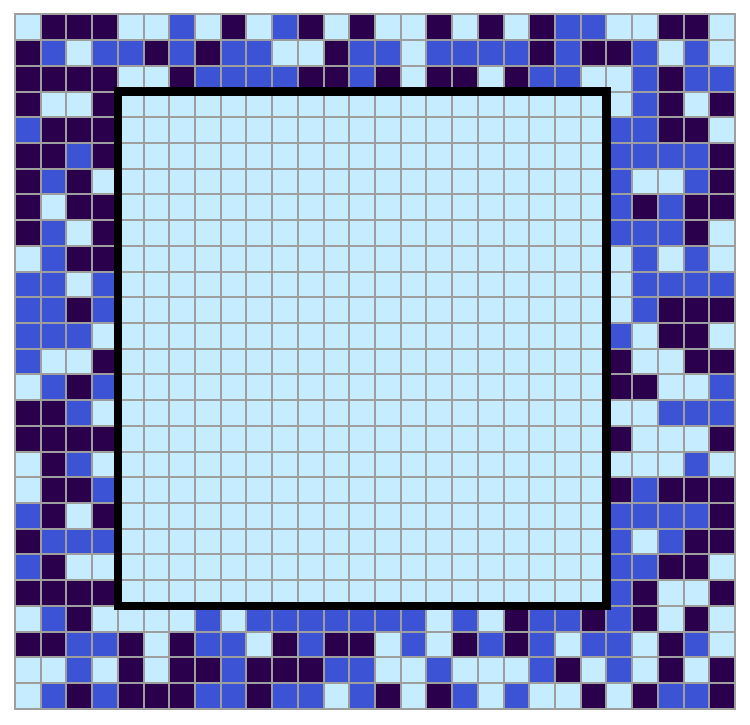
\includegraphics[width=0.45\textwidth]
{AKSs7distM1M2updated}
\end{center}
\caption[]{\label{fig:AKSs7distupdated}
%  AKS 2019-09-10 (Color online)
The site-wise distance \(\Mm_{2,z}-\Mm_{1,z}\) between the $[28 \times
27]$ symbol \brick s $\Mm_{1}$, $\Mm_{2}$ of \reffig{fig:BGcloseActSymb}.
(For a worse visualization, see \reffig{fig:AKSs7dist}.)
}
\end{figure}
%%%%%%%%%%%%%%%%%%%%%%%%%%%%%%%%%%%%%%%%%%%%%%%%%%%%%%%%%%%%%%%%%%%%%%%

\BGpost{2019-08-28} {:
\begin{enumerate}
        \item
\refsect{sect:intro}~{\em Introduction}: there were wide cuts in
comparison to the previous version. This was probably justified, but in
my opinion it is overdone by  now. It is difficult to understand what is
a general motivation for our paper. It looks very technical, dry and
restricted to concrete model.  A bit more poetry on (linear) coding,
e.g.,  why it is useful for description of dynamical systems might
improve things.
        \item
\refsect{sect:overview}~{\em Model and overview of the main results}: I
propose mother figures out how to use LaTex in order how to implement
several of my desired changes in today's so deftly emailed
\texttt{GHJSC16\_notes.pdf} (in yellow).

\end{enumerate}
    }


\PCpost{2019-08-29} {:
\begin{enumerate}
        \item
\refsect{sect:intro}~{\em Introduction}: I would like Boris to write the
general motivation in his own voice, as that is a voice that quantum
chaos community will resonate with. Predrag's pitch in the parallel
\refRef{CL18} universe is to the turbulence community, I think having the
two introductions, sung in different keys, will serve us better.
        \item
Text about not knowing the \PV\ cat map grammar rules is now
moved to just before
\refsect{sect:catLinGreen}~{\em From itineraries to orbits and back}.
\\
\refsect{sect:overview}~{\em Model and overview of the main results}
(Boris yellow markings) is reshuffled, hopefully as was his desire to
have had it reshuffled.
\end{enumerate}
    }


\BGpost{2019-09-07}{redundant, removed:
\\
\textbf{Answer to Q1.}
\textit{
The \catlatt\ admits a natural 2\dmn\  linear symbolic  code with a
finite alphabet. In principle, we can compute analytically the measure of
a given finite {\spt} symbol \brick\ ${\Mm_\R}$ over a region $\R$.
 }
 }

    \PCpost{2019-09-09} {
Files \emph{AKSLPS12\_2.pdf}, \emph{AKSLPS12\_3.pdf} are not referred to
anywhere. If needed, I think they corresponds to log difference of the
two small \twots\ of \reffig{fig:AKScloseActSymb}.
    }

%    \AKSpost{2019-09-10} {
%I have the two {\brick s} $\Mm'_1$, $\Mm'_2$ used to compute
%\reffig{fig:AKSLPS12}\,(b) stored on my laptop and if needed, I can add
%them to the blog.
%\\ \textcolor{blue}{\underline{AKS: taken care of, not needed.}}
%    }

    \PCpost{2017-09-04}{
Border notation in \refeq{inverseq} conflicts with
\refeq{DirichletGreenEquation}. Shouldn't it be
    \(
+\gd_{t,0}\ssp_0+\gd_{t,\ell+1}\ssp_{\ell+1}
    \)
    ?
    }
    \BGpost{2019-09-12}{
No way :)  I checked,  \refeq{inverseq} is correct.
    }
%\BGpost{2019-09-12}{Cannot swallow this:
%   \ie, it connects the partition boundary
%   at time 0 to the partition boundary at time $\ell+1$. }

 \PCpost{2017-09-25}{
Eq.~\refeq{catMapAverCoord} would be ``average coordinate'' for the
periodic boundary conditions, \ie, the periodic point (with repeats of
the defining \brick\ correctly summed. Here $\bar{x}_i({b})$ is at the
lower edge (lower corner?) of the admissible polytope.
    }
%\BG{2019-09-12}{You are right. Changed it to ``approximate coordinate''}


    \BGpost{2019-09-12 }{
I found the calculation following originally upon
\refeq{SingleCatJacobian} redundant, so I removed it to here. Hope you
understand everything without it.

The $\pS_b$ are partitions of the $(\ssp_{0},\ssp_{1})$ \statesp, in
contrast to the polygons $\Pol_{b}$, plotted in the Lagrangian
coordinates $(\ssp_0, \ssp_{\ell+1})$, see \reffig{fig:PairSymbol}. Hence
the interior alphabet measures $\Msr(b)$, $\Ssym{i}\in\Ai$, are given by
the Jacobian \refeq{SingleCatJacobian} of coordinate transformation from
the Lagrangian coordinates $(\ssp_0, \ssp_{\ell+1})$ to the \statesp\
$(\ssp_0,\ssp_1)$,
\(
\Msr(b) = {U_{|b|}({s}/{2})}^{-1}
\,.
\)
The value of $U_{|b|}({s}/{2})$ is always an integer greater than 1,
and thus the $(\ssp_{0},\ssp_{1})$  \statesp\ is ``magnified" and wrapped
around the $(\ssp_0, \ssp_{\ell+1})$ \statesp\ $U_{|b|}({s}/{2})$
times through $\ell$ iterations of the cat map.
Lagrangian coordinates $(\ssp_0,\ssp_{\ell+1})$  are related to \statesp\
coordinates $(\ssp_k, p_{k})$,
\(
p_t = (\ssp_{t} - \ssp_{t-1})/\Delta t \,,
\)
at time $t \in (0, \ell+1)$ by
\begin{eqnarray}
 & x_t &=  \bar{x}_t({b}) +
          \frac{U_{\ell-t}(\frac{s}{2})}{U_{\ell}(\frac{s}{2})}\,\ssp_0
                +
          \frac{U_{t-1}(\frac{s}{2})}{U_{\ell}(\frac{s}{2})}\,\ssp_{\ell+1}
\continue
 & p_\RJedit{{t+1}} &= \bar{x}_{t+1}({b}) -\bar{x}_t({b}) +
          \frac{U_{\ell-t-1}(\frac{s}{2})
               - U_{\ell-t}(\frac{s}{2})}{U_{\ell}(\frac{s}{2})}\,\ssp_0
          +\frac{U_{t}(\frac{s}{2})-U_{t-1}(\frac{s}{2})}{U_{\ell}(\frac{s}{2})}\ \ssp_{\ell+1}
\,.
\nonumber %\label{SquareCut3}
\end{eqnarray}
This is a linear map, so its Jacobian
\(
d_\ell =
   {|\partial (\ssp_0, \ssp_1)}/{\partial (\ssp_0, \ssp_{\ell+1})|}
\)
is simply
\RJedit{
\bea
  d_\ell
%  &=& \frac{\partial (\ssp_0, \ssp_1)}{\partial (\ssp_0, \ssp_{\ell+1})}
  &=& \frac{1}{U_{\ell}(\frac{s}{2})^2}
  \det
   \left(\begin{array}{cc}
  U_{\ell}(\frac{s}{2})  & U_{-1}(\frac{s}{2}) \\
   U_{\ell-1}(\frac{s}{2})  & U_{0}(\frac{s}{2})
  \end{array} \right )
= %\continue &=&
  \frac{1}{U_{\ell}(\frac{s}{2})}
\,.
%\label{SingleCatJacobian}
\eea
}
        }


    \PCpost{2019-09-12 }{Droped this: ``
Unlike the systems studied in \refref{BunSin88}, \catlatt\ cannot be
conjugated to a product of non-interacting  cat maps. A way to see that is, for an example, to
compare the numbers of \po s in the two cases -- they differ.''
    }

            \BGpost{2017-09-14}{
    More  straightforward argument is that $\mathcal{B}_{\scriptscriptstyle L}$ (see
    \refeq{LperHamiltonian} in \refappe{sect:HamiltonCatLatt})  is not
    conjugated to any feline  with  $B=0$).
%    I would not even bring symbolic dynamics issue at
%    this point because symbolic dynamics is a matter of choice. Even if the
%    two maps  are conjugated you can always introduce different/unrelated
%    symbolic dynamics by using whatever partitions.
    }

    \BGpost{2019-09-27}{
Checked \refeq{DirichletGreenEquation}. It is OK. The only question is
whether the notation is sufficiently explained? (I plan to improve a bit
\reffig{fig:block2x2}.)
    }

    \PCpost{2019-09-28} {
% \PC{2019-09-28} rechecked all the blocks
Has anybody checked that the \brick\ of example following
\refeq{2dCatLattAlph7} is admissible?
    }
    \BGpost{2019-09-30} {
Most probably not. On the other hand it is not terribly important. At the
worst case they are all zeroes :)
    }
    \PCpost{2019-10-08} {
Cannot beat the post-Soviet perfectionism :)
    }

        \BGpost{2019-09-30} {
We need Hamiltonian formulation for two reasons. First, our measure
$dp\,dq$ comes from there. Second,  for all   numerics we actually use
initial data problem i.e., Hamiltonian formulation. We need
\refappe{sect:HamiltonCatLatt}, but should keep it compact.
        }

        \BGpost{2019-10-03} {
A risky statement below. Did anybody checked this?
``As $\Xx_{z}$ take rational values for any finite $[L\!\times\!T]$ \twots,
for sites sufficiently close to the center of \R\ the
cancelation $x_{2,z}-x'_{z}$ can be exact.''
{\bf Predrag}: dropped it.
        }

%%%%%%%%%%%%%%%%%%%%%%%%%%%%%%%%%%%%%%%%%%%%%%%%%%%%%%%%%%%%%%%%%%%%%%%%
    \PCpost{2017-01-25} {
Gutkin and Osipov
refer to the map generated by the action \refeq{GutOsi15_3.1:action} as
non-perturbed \textit{coupled cat map},
and to an \twot\ $p$ as a ``many-particle periodic orbit'' (MPO) if
$\ssp_{nt}$ is doubly-periodic, or ``closed,'' \ie,
\beq
\ssp_{nt} = \ssp_{n+L,t+T}
    \,,\quad
n = 0,1,2,\cdots, L-1
    \,,\;\;
t = 0,1,2,\cdots, T-1
    \,.
\ee{GutOsi15po2D}
Action of an \twot\ $p$ is
\beq
S_{p}=-\frac{1}{2}\sum_{t=1}^T\sum_{n=1}^L \Ssym{nt}\ssp_{nt}
\,.
\ee{GutOsi15_3.1:action}
    }
    \BGpost{2019-10-08} {
Do you want  formula for action in the paper?}
    \PCpost{2017-01-25} {
Not unless it is necessary to discuss it anywhere in the paper...
Besides, to me \refeq{GutOsi15_3.1:action} seems almost
surely wrong.}
%%%%%%%%%%%%%%%%%%%%%%%%%%%%%%%%%%%%%%%%%%%%%%%%%%%%%%%%%%%%%%%%%%%%%%%

    \PCpost{2019-01-24}{
    Some of this \twot\ stuff presumably goes to the kittens paper\rf{CL18};
    this paper does only the Dirichlet b.c..
        }
    \BGpost{2019-10-08}{
Do you mean $\gp_{zz'}$? Should we refer here to \rf{CL18} instead of
\refappe{sect:Green}?
    }

        \LHpost{2017-09-05}{
I'm looking at numerical data. The number of total {\admissible} rules of
{cat map} takes an exponential law: $\sim 2.63^n$ for s=3, $\sim 3.74^n$
for s=4 for example. i.e., effectively 2.63/3.74 symbols are needed for
s=3/s=4. They agree with that from the topological entropy and Lyapunov
exponent, which are $(3+\sqrt{5})/2, 2+\sqrt{3}$, respectively.
Intuitively this should hold (that $\log[$~number of {\admissible}
rules]/n = topological entropy), but is it well-known/justified in
symbolic dynamics?
        }
    \BGpost{2019-10-10}{
Now dealt with, in \refsect{sect:catEntropy}. Added concrete numbers to
the picture caption.
    }

%%%%%%%%%%%%%%%%%%%%%%%%%%%%%%%%%%%%%%%%%%%%%%%%%%%%%%%%%%%%%%%%%%%%%%%%
    \BGpost{2017-07-31}
{Should we change layout of \reftab{tab:RJpruning} to the horizontal one? }
    \PCpost{2017-08-11}
{Not sure - easier to see the exponential growth in this format.}
    \LHpost{2017-09-01}{
How about including list of new pruning rules for small lengths as an Appendix?
        }
    \BGpost{2019-09-14}{Would be fine if you can do this.}
%%%%%%%%%%%%%%%%%%%%%%%%%%%%%%%%%%%%%%%%%%%%%%%%%%%%%%%%%%%%%%%%%%%%%%%%

%%%%%%%%%%%%%%%%%%%%%%%%%%%%%%%%%%%%%%%%%%%%%%%%%%%%%%%%%%%%%%%%%%%%%%%%
    \BGpost{2017-08-02} {
\reffig{fig:AKSs13TwoBlock1}
``Any
$4\times 4$ {\brick} of symbols appears one and the same number of times
in both representations.''

means the following: If we scroll/peep  through the
(upper)  torus symbolic representation  with $4\times 4$ window, there
are exactly $NT$ different  $4\times 4$ \brick s of symbols.  Each of
them appears the same number of times, as well,  in the symbolic
representation of the bottom  tori (but for  possibly  different window
positions).
     }
%%%%%%%%%%%%%%%%%%%%%%%%%%%%%%%%%%%%%%%%%%%%%%%%%%%%%%%%%%%%%%%%%%%%%%%%

    \PCpost{2019-10-19}{to Boris and Han:
I have not checked it, but \refeq{SpatiotemporalEntropy} is very pretty,
kind of formula on gets from discrete-Fourier digitalization of Green's
functions. You seem to be saying the $\det$ of the 2-torus Jacobian
matrix counts the numbers of \twots, and are computing $\ln\det$ to get a
rate per area $|\R|$. Could some Chebyshev polynomials lurk  here, and an
analytic answer?
    }

    \PCpost{2017-09-14}{
\catLatt\ metric entropy \refeq{AsymJacobian} is presumably exact for
\catlatt\ as long as \period{} and \speriod{} are going large at
comparable rates. For systems without the space-time symmetry
$t\leftrightarrow{x}$, $h_k$ should be different along the time and
the space directions, so I do not think we can define one spacetime entropy?
Enlightenment on this point would be very welcome.
    }

    \AKSpost{2019-10-20}{to Predrag and Boris:
I can see why we would want to plot the logarithm of the site-wise
distance \(\ln|x_{z}-x'_{z}|\) between the states $\Xx$, $\Xx'$. The idea
would be to remain in the Lagrangian picture. To be clear, right now:
\begin{itemize}
\item
\reffig{fig:BGcloseActSymb} is actually plotting \(\ln \left( \sqrt{(q_z
- q'_z)^2 + (p_z - p'_z)^2} \right) \) which is the site-wise distance in
the Hamiltonian picture ($q = x$ and $p$ is momentum). I already have
generated the figure that corresponds to the Lagrangian site-wise
distance, which is simply  \(\ln|x_{z}-x'_{z}|\). We want that one,
correct?
\item
for \reffig{fig:AKSs13TwoBlock} and \reffig{fig:AKSs13TwoBlock1}, I can
also generate the same 'Lagrangian' distance. For the 3 diamond
blocks, we would have to generate two site-wise distance, let's say
between $(\Xx_1, \Xx_2)$ and $(\Xx_1, \Xx_3)$. Would that work? It would
look something like what's on figure G11 of this blog.
\end{itemize}
\textcolor{blue}{(taken care of by AKS)}
    }

    \PCpost{2019-10-20}{to Boris -
I admit to not understanding to what the title of
\refsect{sect:fullShade}~{\em Full shadowing} refers to. $\Xx_i-\Xx_j$
shadow each other with the doughnuts, as they should, all distances
elsewhere are of O(1). What's {\em Full shadowing} about that?
    }

    \PCpost{2019-10-20}{
I would like to give shelter to \reffig{fig:AKSs13TwoBlock} and
\reffig{fig:AKSs13TwoBlocks1} here in Bloglandia - they would require too
much explanation - and replace them by the likes of
\reffig{fig:AKSdslp12}. We could replace both by a single figure, the
left frame giving \(\ln|x_{z}-x'_{z}|\) for \reffig{fig:AKSs13TwoBlock},
and using \reffig{fig:AKSdslp12} as the right frame, no need to exhibit
the two other pairwise distances, as they should all look very much the
same.

We let Boris decide.
\\ \textcolor{blue}{(taken care of by AKS)}
    }

    \PCpost{2019-10-19} {
Green's function notation is $\gd_{t}$ is not helpful - it's a matrix, so
easier to use $\gd_{tt'}$ throughout.
Green's function notation is $\gd_{nt}$ is not helpful, and here even
misleading - it's a tensorial matrix, so less confusing to use $\gd_{zz'}$
notation throughout.
    }
\BGpost{2019-10-21}
{ Semi-agree :). It is a matter of perception - after all ``Green's
function`` is also (or rather first of all) a function (of $z,z'$).   I
have changed the notation. Looks more clumsy, but might be a less evil.
}

    \PCpost{2016-11-08} {
Say: THE BIG DEAL is

for $d$\dmn\ field theory, symbolic dynamics is not one temporal sequence
with a huge alphabet, but $d$\dmn\ {\spt} tiling by a finite alphabet

``Classical foundations of many-particle
quantum chaos'' I believe could become a game-changer.
Corresponding dynamical zeta functions should be sums over {\twots} (as
is done in the kittens paper\rf{CL18}), rather than $1$\dmn\ \po s.
    }
    \BGpost{2016-11-20} {
All papers that I know were dances around question of uniqueness SRB measure.
Either show that measure is unique or opposite way around (phase
transitions). We know from the start that system is in the high temperature
regime, so the measure is unique.
    }


\BGpost{2019-09-12}{Two remarks
\begin{enumerate}
  \item
In several  cases you call $\Ai$ as a ``full shift''.
This looks wrong. As far as I understand
(see \HREF{http://www.scholarpedia.org/article/Symbolic\_dynamics}
{Scholarpedia}),
one can call $\Ai^\integers$  (together with the shift map $\Tshift$)  as
a ``full shift'', but not $\Ai$. ``Full shift'' is
a dynamical system = state space ($\Ai^\integers$) + map (shift) not just
alphabet.
  \item
Regarding notion of generating partition.
``A partition Q is called a generator or generating partition if
 $\Msr$-almost every point x has a unique symbolic name''.
 So the partitions which we consider here are generating.
 I think what you mean by ``generating''  are  rather called
 ``Markov partitions''.
\end{enumerate}
{\bf Predrag 2019-09-17} Thanks, for me these are very important remarks,
to be fixed also in ChaosBook. Will chew on them... Until then,
keep this remark here, as a reminder.
       }

    \PCpost{2019-10-19} {
I would like to use only one Green's function notation, \ie, $\gp_{zz'}$,
and not $\gd (z,z')$.
    }
    \BGpost{2019-10-19} {
Do you mean $\gd_{zz'}$ ($\gp_{zz'}$ is reserved for periodic boundary
conditions)? I have changed $\gd (z,z')$ to $\gd_{zz'}$, everywhere
except section A3. Seems to me - putting there everything downstairs
would make things  more  uglier.
    }


   \BGpost{2019-09-30}{
To be on the safe side it would be nice to check if everything above is
compatible with numerics on \reffig{fig:RJsymbol}. Is there a hero who
can do this?
    }

     \PCpost{2019-10-20}{
to Boris: A typical reader (if there will be any:)) of this opus magnum
will not be encumbered by precisely your flavor of your quantum chaos
baggage. To motivate this funky section full of peculiar doughnuts and
their permuted holes, you need to explain why action differences (are the
defined anywhere?) need to be small for close \po\ encounters in the
quantum work that connects \po s and quantum chaos spectral
distributions.
    }

\BGpost{2019-10-26}{
It was done already in our paper with Vladimir. No need to repeat.
Motivation here is somewhat different - By using internal symbols you can
easily  manufacture \twots\ with whatever   properties you wish/need (like
in baker's map).
    }

    \BGpost{2019-10-26}{

1) Brought 2 unnamed figures back from the exile  (at least they are correct).

2) Removed some confusion over domains -- $\ZLT$ and $\R$ are 2 different
domains. $\R$ is sub domain of $\ZLT$. Removed some unnecessary/confusing
indexes

3) If you start to change notation (I prefer not to do this  at this
stage) - be careful there is high probability you will need to do it all
over the paper  = lot of work.

4)
Did  not like `doughnut'  slang - everything is pretty flat here (You can
sell some topological stuff  but only after very long and unnecessary :)
discussion = you would need first to make a smooth picture out of this
i.e., discuss smooth field theories. Some attempts in this direction are
in our paper with Vladimir.)   `doughnut hole' is completely misleading.
So for  the lack of anything better I return back to 'annular-like
domain'  = seems to me much less evil.
\\ \textcolor{blue}{(taken care of by AKS)}
    }

    \PCpost{2017-09-06} {to Boris:
Do you have some analytically small number, like $\Msr(\MmR)= 1/8!s(s^2-1)$
for any of the measures in \refsect{sect:2Dnumerics}?
    }
    \BGpost{2019-09-30}
{To Predrag: for this particular $\Mm$  would be a lot of work to get it.}


    \BGpost{2019-10-28}{
Returned \reffig{fig:AKSdslp12} back to Blogosiberia
%%%%%%%%%%%%%%%%%%%%%%%%%%%%%%%%%%%%%%%%%%%%%%
\begin{figure}
\begin{center}
(a) 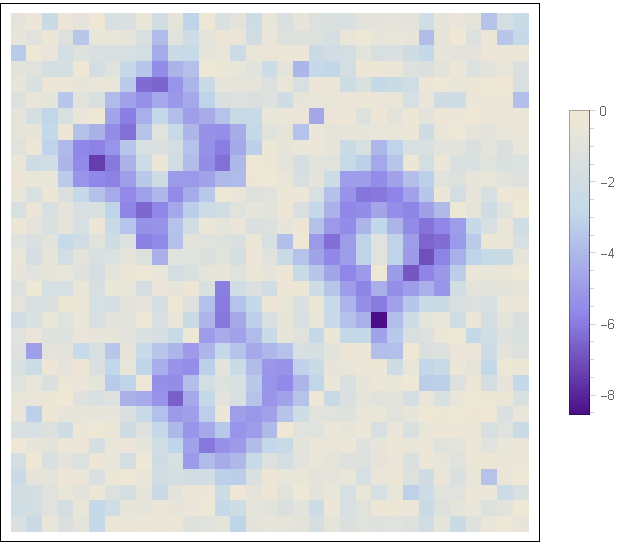
\includegraphics[width=0.45\textwidth]{AKSdslp12}
(b) % \includegraphics[width=0.45\textwidth]{AKS???}
\end{center}
\caption{\label{fig:AKSdslp12}
(Color online) The plots of the logarithm of the site-wise distance \(\ln|x_{z}-x'_{z}|\)
(a) of the states $\Xx_1$, $\Xx_2$ of \reffig{fig:AKSs13TwoBlock}
illustrate the exponential fall-off of the site-wise distances within
the shared doughnut \brick s $\Mm_{\R_1}$, $\Mm_{\R_2}$;
(b) of one of the three pairs of states $\Xx_i$, $\Xx_j$ of
\reffig{fig:AKSs13TwoBlock2}; the other combinations have similar
site-wise distance plots. Outside of the shared domains the distances
are of the order $1$.
    \AKSedit{2019-10-30 Boris: ``completely wrong!''}
    }
\end{figure}
%%%%%%%%%%%%%%%%%%%%%%%%%%%%%%%%%%%%%%%%%%%%%
        }

%    \AKSpost{2019-10-28}{
%Some of the figure referencing has been compromised:
%\begin{itemize}
%\item
%Right now, \reffig{fig:AKSs13TwoBlocks} and \reffig{fig:AKSs13TwoBlocks1}
%refer to appendix figures but should be figures 9 and 11 of the main.
%\item
%The sentence starting with "In figures ... and ... we illustrate these
%parings.." should be figures 9 and 11 of the main and not
%\reffig{fig:AKSs13TwoBlocks} \reffig{fig:AKSs13TwoBlocks1}.
%\item
%The figure mentioned in the caption of figure 11 of the main should be
%\reffig{fig:AKSs13TwoBlock2}. I actually fixed that one. Please approve
%these changes.
%\end{itemize}
%{\bf 2019-10-29 Predrag} Boris seems to have fixed all of these suggestions
%already?
%\\ \textcolor{blue}{(taken care of by AKS)}
%    }

     \PCpost{2017-08-06} {
I have crosschecked \refeq{exactBlock1x1} with
\emph{siminos/spatiotemp/reportRJ.tex}
    }

    \PCpost{2017-09-06} {to Rana - explaining \reffig{fig:RJsymbol} you write:
``relative frequency equal to 0.995755'': how many digits do we trust? we
should state only the significant digits.

 When you replot, and replot you must, make both plots in
\reffig{fig:RJsymbol} square, with both axes going from 0 to 1.
    }

    \PCpost{2016-11-07}{
% Explain in the caption of \reffig{fig:PairSymbol}:
\reffig{fig:SingleCatPartit}:
Note 5th bullet on \refpage{sect:NonlinTips} and \refappe{figinc}.
\\
Refer here (within this comment) to the source code (in the repository) that
generates these figures.
\\
{\bf 2019-10-29 Predrag} giving up waiting on the response.
    }
    \PCpost{2017-09-04}{
to Li Han or Adrien or Rana:
Please reformat the LaTeX layout of \reffig{fig:SingleCatPartit} (not the
plots themselves! and without decreasing the sizes of individual plots)
so each plot has in the lower left corner a label (a), (b), ..., (h), (i)
\\
{\bf 2019-10-29 Predrag} giving up waiting on the response.
        }

    \PCpost{2019-09-30}{
In \reffig{fig:AKSs13TwoBlock} Boris writes ``the two \twots\ $\Xx_1$ and
$\Xx_2$ shadow each other at every point.'' I do not know what ``every
point'' he has in mind, but I agree that $\Mm_1$ and $\Mm_2$ are
identical everywhere except for the $A_1$, $A_2$ permutation, so if I
stand on my head, I can see it being right in some inexplicable sense.

Happy is the referee who grasps \reffig{fig:AKSs13TwoBlocks} without any
reference to any explanatory text.
    }
    \AKSpost{2019-10-28}{
I don't know to what extent do Predrag wanted to explain or define
the use of momentum coordinates in \reffig{fig:AKSs13TwoBlocks} and
\reffig{fig:AKSs13TwoBlocks1}. I
am satisfied with its current state, but could see that we add the
definition for the coordinates $(q^{(i)}_z, p^{(i)}_z)$.
\AKS{2019-10-30}{Those are defined in \refappe{sect:HamiltonCatLatt}}
    }
    \PCpost{2019-10-29}{
Explanation would be nice... When I write in \reffig{fig:AKSs13TwoBlocks}
caption that ``This Hamiltonian representation is explained in
\refappe{sect:HamiltonCatLatt}'' I am lying, no?
\AKS{2019-10-30}{Not sure about that...}
    }

    \AKSpost{2019-10-30}{
Added a \textcolor{blue}{(taken care of by AKS)} note to each completed
blog post which concerned \refsect{sect:twots}.
% I am pretty sure you can remove
% \reffig{fig:AKSdslp12} since Boris said it was completely wrong.
    }

   \RJpost{2019-09-30}{dropped this: ``
If only a column or row of
symbols belongs to the interior alphabet,
the  value of
relative frequency $|\Pol_{\MmR}|$ is typically either  close to $1$ or  $0$.
For example, for
$s=7$
the \brick\
\[
        \left[\begin{array}{cc}
        5 & {3} \\
        \underline{1} & 0
              \end{array}\right]
\,,
\]
with the $[3,0]^T$ column in the interior alphabet,
has a relative frequency $\approx 1-0.005$. % was 0.995755.
''
    }

\PCpost{2016-10-10}{RECHECK! Do they still use pacs?}

     \BGpost{2017-08-31} {
 On my current level of resolution (5 in the morning)
%everything is
%perfect except labels  at x-axis of \reffig{fig:RJsymbol}\,(c) and (d).
%Probably  should be $\gamma -3$ (without 1) under condition you move
%point in \refeq{block2x2bases=3} one step right.
%%Also word ``decimal" should be erased from the earth (or at least from
%%the caption and near \refeq{block2x2bases=3}.
%% On p. 6 (down) probably ``requires AN extensive use  of ..."
%Otherwise
the paper is completely ready for submission  at any journal of this
galaxy.
    }
\end{description}

\subsection{Cats/nonlin-v2/  GHJSC16 revisions}
\label{sect:GHJSC16blogV2}
\begin{description}

     \BGpost{2020-10-16} {dropped formulas\\
The remarkable feature of the {\catlatt}  is that its every solution
\(
\{\ssp_{z},  z\in \integers^{d}  \}
\)
is uniquely encoded by a linear transformation to the corresponding finite
alphabet $d$\dmn\ symbol lattice
\(
\{\m_{z}, z\in \integers^{d}\}
\)
    }

     \BGpost{2020-10-16} {dropped formulas\\
dropped:\\
This paper builds explicit 2\dmn\ {\catlatt} \statesp\ partitions using
winding numbers  \(\m_{z}\). An alternative, generating \AW\ partition
for the cat map, and a \po\ theory for \catlatt\ in higher dimensions are
formulated in the parallel paper\rf{CL18}.

inserted instead later:\\
\edit{
This paper builds explicit 2\dmn\ {\catlatt}   symbolic dynamics  using
winding numbers  \(\m_{z}\). (An alternative construction, based on
generating \AW\ partition for the cat map, and a \po\ theory for
\catlatt\ in higher dimensions are formulated in the parallel
paper\rf{CL18}.)
    } %end \edit
        }

     \PCpost{2020-10-17} {
Removed:\\ ``(An alternative construction, based on  generating \AW\ partition
for the cat map, and a \po\ theory for \catlatt\ in higher dimensions are
formulated in the parallel paper\rf{CL18}.)''

The case $s<-\edit{2}$ can be treated analogously.
        }

     \BGpost{2020-10-16} {added:\\
\edit{
The following theorem allows  for evaluation of symbol blocks measures.
\begin{theorem}
Let $b$ be a finite sequence of symbols.  The corresponding  measure  is
given by the product
\beq
 \Msr({b}) =d_\ell |\Pol_{b}|,  \qquad  d_\ell =
  {1}/{U_{\ell}({s}/{2})},
\ee{FreqDecompBlog}
where
 $|\Pol_{b}|$ is  the area of the polygon $\Pol_{b}$
defined  by the inequalities
\begin{eqnarray}
 & 0&\leq \bar{x}_i({b})
     +\frac{U_{\ell-i}(s/2)}{U_{\ell}(s/2)}\ssp_0
     +\frac{U_{i-1}(s/2)}{U_{\ell}(s/2)} \ssp_{\ell+1}<1
     \,,\qquad i=1,\dots ,\ell,
\label{SquareCut1blog} \\
 & 0&\leq \ssp_0 <1, \qquad  0\leq \ssp_{\ell+1} <1
 \,
\label{SquareCut2blog}
\end{eqnarray}
in the plane $(\ssp_0,\ssp_{\ell+1})$.
\end{theorem}
    }
} %end \edit

     \PCpost{2020-10-16} {
Boris has now renamed  refeq~{FreqDecomp} to \refeq{FreqDecomp1}. While
Boris-introduced \refeq{FreqDecomp} is cited many times, \refeq{FreqDecomp1}
is never cited.

Too many `In general,'s

mark as EDITED:\\
Since all coefficients in  (\ref{SquareCut1})  are given by rational numbers,
the polygon areas $|\Pol_{{b}}|$ are rational too. The same holds for the
$d_\ell$ factor. As a result,   measures  $\Msr({{b}})$ are always rational
(see, for example, \reftab{tab:RJ2letFreq}). This allows for their exact
evaluation by integer arithmetic.  As the factor $d_\ell$ in \refeq{FreqDecomp} is known explicitly, the
    }

     \BGpost{2020-10-16} {rewrote:
\paragraph{Interior symbols.}
For \brick s composed of interior symbols only, the inequalities
(\ref{SquareCut1})  are always satisfied, and  $\Pol_{{b}}$ are unit
squares of area $1$. The corresponding measure
\[
\Msr({b})
= {1}/{U_{|{b}|}({s}/{2})}, \qquad  \Ssym{i}\in \Ai
\,, \quad  i=1,\dots |{b}|
\]
depends  only  on the length of the \brick\ ${b}$.

\paragraph{Rationality.}
Since all coefficients in  (\ref{SquareCut1})  are given by rational numbers,
the polygon areas $|\Pol_{{b}}|$ are rational too. The same holds for the
$d_\ell$ factor. As a result,   measures  $\Msr({{b}})$ are always rational
(see, for example, \reftab{tab:RJ2letFreq}). This allows for their exact
evaluation by integer arithmetic.
    }

     \PCpost{2020-10-31} {
Dropped: `` The always trustworthy but so un-cited Soviet scientists
(1781–1840) teach us that...'
    }

     \PCpost{2020-10-17} {
Edited everything down to $d=2$ dimensions. Was:\\
The \templatt\ map \refeq{eq:CatMapNewton1}, and the \catlatt\
\refeq{eq:CatMapNewton2} can be brought into uniform notation  and
generalized  to $d$ dimensions by converting the {\spt} differences to
discrete derivatives. This yields the discrete screened Poisson
equation\rf{Dorr70,HuCon96} for the $d$\dmn\ {\em \catlatt}.

The key insight  is that  {\em $d$\dmn} {\spt}
 lattice of integers
\(
\{\m_{z}\} = \{\m_{z}, z\in \integers^{d}\}
\)
is the natural encoding of a $d$\dmn\ {\spt} state.

Eq.~\refeq{LinearConn} was
\bea
 (-\Box +\edit{2(s-2)})\,\ssp_{z} &=& \Ssym{z}
\,,\qquad
  \Ssym{z} \in \A
\,,
\continue
 && \A = \{-2d+1, -2d+2,\cdots,s-2,s-1\}
\,,
\label{LinearConnBlog}
\eea
            }

    \BGpost{2020-11-12}{
With the redefined stretching parameter ${s}$ alphabet runs up to $2{s}-1$.
${s}$ can attain half-integer values.
    }
    \PCpost{2020-11-15}{
Thanks for noticing that $\A = \{-3, -2,\cdots,s-2,s-1\}$ in
\refeq{LinearConn} was not updated to \refeq{CoupledCats}. Fixed now.
Yes, ${s}>2$ can attain half-integer values, the lowest one is ${s}=5/2$.
    }

    \PCpost{2020-11-15}{
I do not remember the unnumbered equation after \refeq{msrMmR} any
longer. Do I know this identity? Does it follow from Green's function
being the inverse of the linear operator in \refeq{CoupledCats}? From
\refappe{sect:Green2Dident}~{\em Lattice Green's identity}? I changed it
to $2(s-2)$ rather than the old convention $(s-4)$.
    }

    \BGpost{2020-11-12}{
Text below \refeq{relFreqNew} -
``from which the above `generic' state X is assumed to be drawn.''\\
This part is very unclear. To obtain a generic solution X you need to
draw  generic (with respect to mu) initial conditions and then apply the
map which is defined  in the appendix. This how we check our results
numerically.
    }
    \PCpost{2020-11-15}{
Ok. Go ahead with the rewrite.
    }

    \BGpost{2020-11-12}{
Have we defined \R\ before the end of ``Answer to Q1"?
    }
    \PCpost{2020-11-15}{
Yes, see 4 lines above \textbf{Q1.}.
    }

    \BGpost{2020-11-12}{
$\edit{s=2}$ is the marginal case, with one zero Lyapunov exponent.
Apparently  the results are applicable  to this case as well, as numerics
shows.
    }
     \PCpost{2020-10-17} {
In \reffig{fig:RJsymbol} we are simulating the marginal, $\edit{s=2}$
(Laplace operator) case. I do not trust student's simulations here -it's
so easy to miss power laws- but it's too late to do anything about that.
We will pass it over in silence, unhappily.

{\color{red}{\qquad To
Boris: This Dirichlet bc is lots of pain for a no gain. Again I do not
know what even $\R=[1\time1]$ means. Or Figure 4.~(a) A $[5\times3]$
domain \R\ I would like to think of as a $[4\times2]$ domain, centered on
$(\ell_j+1)/2$. Will rethink this tomorrow. For now, Good night.
}}
    }


\end{description}
